%% =====================================================================
%% CIM Roofline Model -- second restructured edition (window-based Q_R)
%% ---------------------------------------------------------------------
%% Companion to roofline.tex.  Two core changes over the previous edition:
%%
%%   1. Q_R is redefined over a steady-state analysis window W:
%%        Q_R(W) := bytes that traverse the resident channel inside W,
%%      where W is one representative repetition unit of the workload
%%      under stable, steady-state operation (one inference event,
%%      one decode step, one training step, one token KV append, ...).
%%      This resolves the inconsistency in the earlier edition where
%%      “unique resident bytes” was used as Q_R while the main
%%      formula P <= min(rho, tau*RI) implicitly required “bytes
%%      actually traversing the resident channel”.
%%
%%   2. All concrete numerical calibrations of (rho, tau, Q_S, Q_R)
%%      are concentrated in Section 5.  Sections 4 and 6 stay
%%      qualitative and refer back to Section 5 for specific values
%%      rather than re-citing calibration numbers across the text.
%%
%% The structure otherwise follows roofline.tex and preserves all
%% \label names so cross-document references remain valid.
%% =====================================================================

\documentclass[11pt, a4paper]{ctexart}

%% --- Mathematics ----------------------------------------------------
\usepackage{amsmath, amssymb, amsthm}
\usepackage{mathtools}
\usepackage{bm}

%% --- Tables and layout ----------------------------------------------
\usepackage{booktabs}
\usepackage{array}
\usepackage{tabularx}
\usepackage{multirow}
\usepackage{makecell}

%% --- Page geometry --------------------------------------------------
\usepackage[margin=2.5cm]{geometry}
\usepackage{setspace}
\setstretch{1.15}

%% --- Line-breaking for mixed CJK + Latin text ----------------------
%% Half-width punctuation (used throughout this file) does not provide
%% xeCJK break opportunities; the resulting long Latin runs with embedded
%% citations/units can overflow the right margin. Allow LaTeX to stretch
%% inter-word space up to 3em to find acceptable line breaks.
\setlength{\emergencystretch}{3em}

%% --- Typography -----------------------------------------------------
\usepackage{microtype}
\usepackage{xcolor}
\definecolor{gpuColor}{RGB}{30, 80, 180}
\definecolor{cimColor}{RGB}{190, 40, 40}
\definecolor{emphColor}{RGB}{140, 50, 140}

%% --- Disable italic Kaiti ------------------------------------------
%% ctex binds the italic/kaishu slot of CJK text to STKaiti by default.
%% We eliminate KaiTi from the document in three layers:
%%   (1) redirect all italic-like command-level semantics to bold
%%   (2) override \kaishu / \fangsong to fall back to \songti
%%   (3) rebind the CJK italic font slot itself to STSong, so that
%%       even internal NFSS shape switches cannot reach STKaiti
\let\emph\textbf
\let\textit\textbf
\renewcommand{\itshape}{\bfseries}
\renewcommand{\kaishu}{\songti}
\renewcommand{\fangsong}{\songti}

%% Layer (3): override the CJK italic slot at the font-binding level.
\setCJKmainfont{STSong}[
  ItalicFont     = STSong,
  BoldFont       = STHeiti,
  BoldItalicFont = STHeiti
]
\setCJKsansfont{STHeiti}[
  ItalicFont     = STHeiti,
  BoldFont       = STHeiti,
  BoldItalicFont = STHeiti
]

%% --- Figures --------------------------------------------------------
\usepackage{graphicx}
\usepackage{tikz}
\usetikzlibrary{arrows.meta, positioning, calc, decorations.pathreplacing}
\usepackage{float}  % allows [H] specifier for in-place tables/figures

%% --- Hyperlinks -----------------------------------------------------
\usepackage{hyperref}
\hypersetup{
  colorlinks=true,
  linkcolor=blue!55!black,
  urlcolor=blue!55!black,
  citecolor=blue!55!black
}

%% --- Captions -------------------------------------------------------
\usepackage[small, bf, hang]{caption}

%% --- Lists ----------------------------------------------------------
\usepackage{enumitem}

%% --- Theorem environments ------------------------------------------
%% Force “definition” style (upright body) for ALL theorem-like envs,
%% so that Chinese body text is never rendered in italic (which ctex
%% would otherwise substitute with KaiTi).
\theoremstyle{definition}
\newtheorem{definition}{定义}[section]

%% --- Custom commands -----------------------------------------------
\newcommand{\unit}[1]{\,[\mathrm{#1}]}
\newcommand{\AI}{\mathrm{AI}}
\newcommand{\RI}{\mathrm{RI}}
\newcommand{\QS}{Q_{S}}
\newcommand{\QR}{Q_{R}}

%% --- Title ---------------------------------------------------------
\title{\bfseries 存算一体架构下的 Roofline 模型 \\[0.3em]
\large 从硬件分解到操作数角色分解}
\author{}
\date{\today}

\begin{document}
\maketitle

%% ===================================================================
\begin{abstract}
\noindent
经典 Roofline 模型~\cite{williams2009roofline} 以\textbf{算力} $\pi$ 与\textbf{带宽} $\beta$ 作为计算平台的两个关键指标, 以\textbf{计算量}与\textbf{访存量}作为网络模型的两个关键指标, 在冯诺依曼架构下形成了一个量纲对称、可视化清晰的性能上限分析框架。然而一旦进入存算一体 (Compute-in-Memory, CIM) 架构, Roofline 所依赖的全部物理前提 (存算硬件分离、数据同质化、compute-memory 二元瓶颈结构) 同时失效。直接照搬或零散修补经典 Roofline 都会与底层物理事实结构性不一致。

本文从第一性原理重新构建 CIM 的 Roofline。核心洞察是: \textbf{GPU 与 CIM 在底层反转了 “异构维度”}。GPU 是\emph{异构硬件}处理\emph{同质数据}, CIM 是\emph{同质硬件}处理\emph{异构数据}。这一反转使得 Roofline 的坐标轴必须按\emph{操作数角色} (resident 与 streaming) 分解, 而非按\emph{硬件功能} (compute 与 memory) 分解。

由此导出一对新硬件指标: $\rho$ (流式数据吞吐) 与 $\tau$ (驻留数据吞吐); workload 侧引入\emph{稳态分析窗口} $W$, 按窗口给出 $Q_S(W)$ (窗口内经 streaming 通路的字节) 与 $Q_R(W)$ (窗口内经 resident 通路的字节, 包含 attention 的 KV append、训练的权重回写、容量不足导致的权重重装等); 进而引入无量纲驻留强度 $\RI = Q_S/Q_R$ (Resident Intensity), 给出 CIM Roofline 公式
\[
P \;\le\; \min\!\bigl(\rho,\ \tau\cdot\RI\bigr)\quad [\mathrm{Byte}/\mathrm{s}].
\]
两个受限分区分别为\textbf{驻留吞吐受限} (resident-bound, 算法 $\RI$ 过低) 与\textbf{流式吞吐受限} (streaming-bound, 算法 $\RI$ 充分)。按窗口内是否触发 resident 通路写入, workload 自然划分为\emph{静态驻留} ($Q_R(W) = 0$, Roofline 退化为 $P \le \rho$) 与\emph{动态驻留} ($Q_R(W) > 0$, regime 由 $\RI$ 与脊点 $\RI^{*} = \rho/\tau$ 比较决定) 两类工况; 硬件容量与器件耐久度可在公式之外限制实际可达的工作点 (例如小容量阵列上推理大模型会被强制进入持续重写, 把名义为静态驻留的 workload 推入动态驻留)。

基于 28\,nm CMOS 外围电路基线, 对 SRAM ACIM/DCIM、Gain Cell、FeNOR、FeRAM、RRAM、NOR Flash、3D NAND TLC 七类 CIM 技术给出 $(\rho, \tau, \RI^{*})$ 的解析估算; 对 LLM 主要 workload 按窗口给出 $(Q_R, Q_S, \RI)$ 的解析; 二者构成 “硬件 $\times$ workload” 二维 regime 矩阵。主要发现包括: 训练与 KV-append decode 在主流 CIM 技术上都是流式吞吐受限 (而非 GPU 视角下惯常预期的存储受限), FeNOR 的 $\RI^{*}$ 与 LLM 动态 workload 数值天然吻合, RRAM 与 NOR Flash 本质上只适合一次烧入的静态部署, 3D NAND 不止适合静态推理且对训练与长上下文 decode 也能进入流式吞吐受限带。

作为应用, 框架直接给出\textbf{端侧 LLM CIM 推理采用 PD 融合}的 Roofline 级判定: GPU 上 PD 分离的两条独立依据 (资源分裂架构、P 与 D 跨 regime) 在 CIM 上同时失效, P 与 D 落在同一 regime 带; 双硬件分离方案令窗口内 $Q_R(W)$ 翻倍、$\RI$ 减半、工作点漂移驻留吞吐受限带, 模式切换分离方案令切换时间累积成为可测的稳态性能损失; 理论与工程两层同时指向 PD 融合是 CIM Roofline 的自然推论。

在更深层次上, 本文指出经典算法分析里 “时间复杂度对空间复杂度” 的对偶其实是冯诺依曼架构的特化投影; CIM 给出同一底层对偶的另一种具体形式: “流动复杂度对驻留复杂度”。两套 Roofline 由一个\textbf{通道分解原理}统一生成: 任何架构的性能上界由其独立服务通道中最慢的一条决定, 通道集合由架构异构维度决定。GPU (资源分裂、角色合并) 与 CIM (角色分裂、资源合并) 是该原理在两种正交异构选择下的两个投影。
\end{abstract}
\newpage

%% ===================================================================
\section{引言}
\label{sec:intro}

经典 Roofline~\cite{williams2009roofline} 已是加速器性能分析的标准工具，近年来被广泛沿用于存算一体 (CIM) 性能评估~\cite{liu2025ar_llm,sharma2025wwwtocim,zhou2025imcsim}。然而把它应用到一块 CIM 阵列上，会立即遇到三个无法回避的问题：

\begin{enumerate}[topsep=2pt, itemsep=2pt]
  \item \textbf{“算力”无处赋值}。经典 Roofline 把“compute 单元每秒能做多少 OP”作为一个独立硬件指标 $\pi$。在 CIM 阵列里，MAC 不是某个计算硬件\emph{执行}的动作，而是权重和输入共同到位后由欧姆定律 $+$ 基尔霍夫电流定律\emph{涌现}的瞬时结果——没有可被独立赋速率的“compute engine”。
  \item \textbf{“带宽”不止一条}。CIM 上数据有两类入口：权重经编程通路缓慢写入 cell，输入经 DAC--WL--BL--ADC 通路高速通过阵列。这两条通路物理独立、速率与延时相差几个数量级，无法合并成单一标量 $\beta$；若同时保留多个，Roofline 的“二维简洁”不再成立。
  \item \textbf{“访存量”失去定义}。经典 $\AI = \mathrm{OP}/\mathrm{Byte}$ 的分母默认所有数据无差别；但在 CIM 上权重(一次写入服役整个推理)与激活(每 token 流过)走的不是同一通路、字节意义不同，无法一律计入“访存量”。
\end{enumerate}

这些不是命名问题，也不是 CIM 体系尚不成熟才出现的瑕疵。它们指向一个事实：Roofline 的整套形式背后是\emph{冯诺依曼专属的}三条架构前提——存算硬件分离、数据同类化、compute-memory 二元瓶颈结构。CIM 同时违反这三条。任何“在 $\pi/\beta$ 框架内打补丁”的尝试，本质上都在用一种架构的指标语汇描述另一种架构的物理事实，只能得到与底层物理不一致的结论。

解决该问题的关键不在于构造更复杂的公式，而在于辨识 GPU 与 CIM 的本质差异：两者\textbf{把“异构性”放在了不同维度}。GPU 是\emph{异构硬件}(compute 单元 $\neq$ memory 单元)$\times$\emph{同质数据}(权重/激活/中间值都是 Byte)；CIM 是\emph{同质硬件}(阵列处处是 MAC)$\times$\emph{异构数据}(resident vs streaming 走两条物理路径)。两者互为对偶。沿这一对偶反转，Roofline 的形式逻辑可\emph{反方向投影}到 CIM：将任务量的分解原则从“按硬件功能”改为“按操作数角色”。

本文沿这条路径系统重构 CIM 的 Roofline。第~\ref{sec:background} 节复述 GPU Roofline 并显式提出其三条架构前提。第~\ref{sec:insight} 节展示 CIM 如何系统性违反这三条前提、为何必须更换分解维度，并将工作量单位从 OP 转向 Byte。第~\ref{sec:cim_roofline} 节构建 CIM-native 的硬件、模型、强度、公式与几何，并补足稳态窗口、pipeline 实现机制、工况模式分类、与 GPU Roofline 的对偶、架构间坐标变换、容量修正这一整套配套结构。第~\ref{sec:quantitative} 节将符号代入 28\,nm CMOS 基线得到具体数字，给出“硬件 $\times$ workload”二维 regime 矩阵并验证主流工程直觉。第~\ref{sec:pd_fusion} 节应用框架推出“端侧 LLM CIM 推理采用 PD 融合”的明确结论。第~\ref{sec:channel_decomposition} 节将两套 Roofline 统一为同一通道分解原理的两种投影，并由此重新审视“时空对偶”的本质。第~\ref{sec:conclusion} 节给出总结与展望。

\newpage

%% ===================================================================
\section{GPU Roofline 回顾及其三条架构前提}
\label{sec:background}

本节先回顾 Roofline 的提出动机与现有 CIM 评估工作的应用现状（第~\ref{sec:roofline_review} 节），随后复述经典 Roofline 的形式化定义。目的不在于重申已知公式，而在于将其依赖的\textbf{三条架构前提} (P1)--(P3) 显式提出，作为第~\ref{sec:insight} 节系统性审查的参照。

\subsection{Roofline 的提出与在 CIM 上的应用现状}
\label{sec:roofline_review}

在进入 GPU Roofline 的形式化复述之前，本节先回顾 Roofline 这一工具的提出动机、十余年来的主要延伸路线，以及近年研究者把它搬到 CIM/IMC 平台上时所采取的具体姿态。其目的有两点：其一，把 Roofline 的核心价值与其默认的架构前提显式区分开，为后续 (P1)--(P3) 的提炼提供文献依据；其二，整理现有 CIM-Roofline 工作在 “是否分离权重字节与激活字节、是否把权重写入纳入公式、是否承认 ADC/peripheral 的特殊地位” 等关键问题上的处理差异，让本文 “换坐标系” 而非 “在 $\pi/\beta$ 框架内打补丁” 的选择有清楚的对照背景。

\paragraph{Roofline 的提出：多核时代的可视化语言}
Roofline 由 Williams、Waterman 与 Patterson 于 2009 年提出~\cite{williams2009roofline}，直接动机是多核架构的快速分化（核心数、缓存层级、本地存储、异构核如 IBM Cell）让程序员、编译器与架构师都难以对齐性能直觉。作者并不追求精确的统计或概率预测，而是借用 Lazowska 等人的 bound-and-bottleneck analysis 传统，给出一个 “易理解、可视化、不必精确但要有洞察力” （原文：“easy-to-understand, insightful, not perfect”）的上界模型。其核心抽象只有三个量：峰值算力 $\pi$、峰值 DRAM 带宽 $\beta$，以及 operational intensity $\AI = \mathrm{OP}/\mathrm{Byte}$；二者经二元 $\min$ 归约得到 $P \le \min(\pi,\ \beta\cdot\AI)$，在 $\AI$--$P$ 平面上呈 “ceiling 加 slope 加脊点” 几何，划分 compute-bound 与 memory-bound 两个分区。

Williams 等人在原文中已经显式给出了 Roofline 的两条隐含假设：算力与带宽对应物理上分离的两个客体，DRAM 通路是数据进入计算的唯一入口。他们也提出可以用 L2 带宽或 I/O 带宽替换 DRAM 带宽以得到 “different rooflines”，但讨论范围始终限定在冯诺依曼缓存-多核架构上，没有涉及 PIM、analog compute 或本文关心的存算一体。文中也强调 Roofline 的几何形态——ceiling 加 slope 加脊点——是这两条假设的直接产物，而非 Roofline 抽象自身的必然性，这一观察对本文重构 CIM Roofline 尤为关键。

\paragraph{在 $\pi/\beta$ 框架内的延伸}
过去十余年，Roofline 已成为加速器性能分析的事实标准，也被持续扩展以适配新的架构形态，但所有延伸都保留了原版的 $\pi/\beta$ 二元结构。Rheindt 等人 2020 年的综述~\cite{rheindt2020xcentric} 把现代体系结构划分为 compute-centric、memory-centric 与 application-centric 三族，把 in-memory 与 near-memory computing 都归入 memory-centric，并指出 Roofline 在异构多 PE 系统下需要扩展为 Gables 风格的多 Roofline 叠加（每个 PE 一条独立 Roofline）；但作者也在该综述中承认 “a programming paradigm specific to memory-centric systems is missing”，对 CIM 的特殊物理只在调研层面提及，并未给出新形式。

Verhelst、Benini 与 Verma 2025 年在 IEEE JSSC 上的工作~\cite{verhelst2025roofline} 正面回应 vanilla Roofline 在现代 ML 加速器上的不足，把 Roofline 系统地扩展为一套面向 ML 加速器设计空间的工具。出发点是 ML 模型规模过去十年以约 100$\times$/24 个月扩张、远超摩尔定律，加速器设计必须同时调用并行化、空间-时间复用、量化、稀疏、近存/存内计算等多种手段，而单一 Williams Roofline 难以联合刻画这些手段。他们由此引入两项核心扩展：其一是按存储层级展开的 hierarchical Roofline $P_{\mathrm{TP}} = f_{\mathrm{clk}} \cdot \min(\AI_{L_1} \cdot B_{L_1}, \ldots, \AI_{L_n} \cdot B_{L_n}, A_{\mathrm{op}})$（其文中 Eq. 4），因为 NN 在不同存储层级上的 $\AI$ 差异显著、不能压缩为单一带宽；其二是引入与吞吐 Roofline 并列的 energy Roofline $P_E = 1/(E_{\mathrm{op}} + \sum_i E_{L_i}/\AI_{L_i})$（Eq. 5），其拐点位置一般与吞吐 Roofline 不同，使一个 workload 可同时处于吞吐 compute-bound 与能效 memory-bound，从而显式区分 “为吞吐设计” 与 “为能效设计” 两个目标。

对 IMC 这一架构，Verhelst 等人有专门讨论。他们把 IMC 描述为 “2-D 空间架构的极端情形”，指出 IMC 在 bit cell 一级耦合 storage 与 compute、权重直接驻于阵列、不再走 first-level memory，因此 first-level memory 对应的 Roofline 对角线被 “消除”；在他们的多层 Roofline 上，IMC 的好处即编码为两件事：抬高 compute-bound ceiling，并把 workload 工作点系统地推向计算受限带。他们也直接点出 IMC 的核心张力：IMC 同时融合 storage 与 compute，但一旦想分别优化两者的利用率（例如 fully-weight-static mapping），融合反而成了约束——即 “IMC intrinsically couples storage and compute resources, yet maximizing utilization and scalability requires optimizing each of these separately. This prevents a fully-weight-static workload mapping”。

可以看到，Verhelst 等人对 IMC 的处理相当深入，且已经识别出 storage-compute 耦合所带来的优化困难。但他们的所有修正——多层级、能效、IMC 单独标注——都仍在 $\pi/\beta$ 二元结构内展开（纵轴仍是 OP/s 或 TOPS/W、横轴仍是 OP/Byte），并没有更换分解维度本身。本文与他们之间的根本区别即在这里：本文不再尝试在 $\pi/\beta$ 框架内表达 CIM，而是把分解维度本身从硬件功能改为操作数角色。

\paragraph{直接照搬 GPU Roofline 分析 CIM 的工作}
近年研究者把 Roofline 直接搬到 CIM 系统的工作可分为若干姿态，最常见的一类是不修改 Roofline 形式、仅把 CIM 当作 “一种新的存储或计算硬件”，把 $(\pi, \beta)$ 重新赋值后画 Williams 形式的 $\AI$--$P$ 图。

Liu 等人 2025 年讨论端侧 AR SoC 上 LLM 推理的工作~\cite{liu2025ar_llm} 是这一姿态的典型代表：他们在 TOPS vs Ops/Byte 与 TOPS/W vs Ops/Byte 两张 Roofline 上同时绘制 LPDDR5X 基线、DRAM-PIM、SRAM-CIM、3D-DRAM 四种存储方案，并按 GPU 视角得出 “Llama3 Prefill 算力受限、Decode 存储受限” 的工况判定。Sharma 等人 2025 年的工作~\cite{sharma2025wwwtocim} 把 algorithmic reuse $\equiv 2MNK/(MN + NK + MK)$ 定义为算术强度，沿用 “low arithmetic intensity GEMMs are limited by the memory bandwidth, while high arithmetic intensity GEMMs are limited by the peak performance” 这一典型 GPU 表述，对 SRAM-based CIM 在 GEMM workload 下做能效与吞吐评估。Sun 等人 2023 年从 AIMC 与 DIMC 的 component-level 量化建模出发~\cite{sun2023imc_benchmark}，把 “roofline” 仅作为峰值上界的同义词使用（原文：“peak performance is the starting metric for evaluation as it provides a roofline for the computational capabilities of the design”），这种降格使用等于隐含承认了经典 Roofline 不足以刻画 CIM 的实际性能动态。Zhou 等人 2025 年的 IMCsim 仿真器~\cite{zhou2025imcsim} 输出经典 Roofline 图来对比 ResNet-18、Llama 6.7B、DiT-XL/2 在三种 IMC 处理器上的位置，但他们自己的实验同时给出一个反例：Llama 在 Roofline 上被判 memory-bound，通过重塑 bank 维度（把 row 数从默认的 512 改为与 quant group 匹配的 128）仍可获得近 8$\times$ 的实测加速——也就是说 Williams Roofline 给出的 regime 诊断在 CIM 上不可靠。

上述四项工作的共同点是：把 CIM 当作一种 “$\pi$ 更高、$\beta$ 更高、energy 更低的新硬件”，在 GPU Roofline 坐标系里重新画线，但保留 “按硬件功能分解任务量” 这一根本前提。这种做法会立即产生几个内部张力，后文 “共性局限” 一段集中陈述。

\paragraph{尝试改写 Roofline 形态的工作}
另一些工作意识到经典 Roofline 在 CIM 上的形态不对，尝试做局部修正，但都没有把 “分解维度” 这一根本问题摆上台面。

最早的线索可以追溯到 Verma 等人 2019 年的 IMC 综述~\cite{verma2019imc}。他们在论述 IMC 动机时使用 Roofline 作为概念图，提出 “loading-bound” 与 “compute-bound” 的划分，并明确指出 “while IMC reduces the costs of MVM computation, it doesn't change the costs of loading data in the memory circuits; thus, gains are derived only if MVM computation costs dominate at the system level”——这一判断与本文 “streaming-resident 二元归约” 的核心直觉一致。但他们的 Roofline 使用是粗略的，两轴均为 OP/s 单位，没有形式化的强度概念，也没有把 ADC、peripheral 这些 IMC 特有的瓶颈纳入坐标。

Jia 等人 2022 年在 IEEE JSSC 上给出的可编程 IMC 推理加速器~\cite{jia2022imc_accelerator} 是本文方向上最早、也是结构上最接近的一项工作。他们的原型在 16 nm CMOS 工艺下实现 4$\times$4 个 CIMU (compute-in-memory unit) 的阵列；每个 CIMU 内含一个 1152 行 $\times$ 256 列电容耦合混合信号 CIMA (compute-in-memory array)、两个数字 SIMD 引擎（BPBS SIMD 用于多 bit 计算的 bit-parallel/bit-serial 重构，CMPT SIMD 用于激活、缩放、池化等元素级与跨元素运算）以及输入/shortcut 缓冲；CIMU 之间通过片上互联 (OCN) 交换激活，由独立的权重加载 (WL) 网络从外部 SRAM 写入权重。原型 4$\times$4 CIMU 整阵列峰值约 3 TOPS、30 TOPS/W (8 bit)，CIMU 数量本身可按面积与吞吐目标缩放、不固定。这一架构本身已经把 IMC 系统的物理资源拆分为 “阵列计算 + 权重写入 + 激活搬运 + 近存 SIMD” 几条并行通路，他们在性能分析里也对应地没有沿用 GPU Roofline 形式。

他们的 Roofline 图（论文 Fig. 2）把横轴改为 “compute intensity per weight”——即每写一次权重在 IMC 阵列里支撑多少次 MAC，把纵轴的可达吞吐分为两个明确的 regime：\textbf{IMC-write-bound} 与 \textbf{IMC-compute-bound}。物理直觉清晰：每次将权重写入 CIMA bit cell 都要付出可观能量与时间，因此只有当每次写入被很多次 MAC 复用时，IMC 的高密度算力才能摊销 write 代价；当复用度不足，瓶颈从阵列计算转向权重写入。文中 Table I 给出一个关键的数量级对比：IMC 的 write 与 MAC 能耗之比约 $30\times$，远超数字加速器对应的约 $2\times$——正是这一不对称使 write 通路在 IMC 上需要被单列为一条独立 Roofline 受限分区，而在数字架构里通常无需如此。基于这一 Roofline，他们扫描了多种 mapping 与系统规模，并观察到一个非平凡的副结果：随阵列规模扩大、复制权重以提升并行度，每权重支撑的 MAC 数反而下降，工作点被推向 IMC-write-bound 一侧——即 “the typical approach of data-level parallelism (also known as replication) directly reduces data reuse below the maximum”。

Jia 等人这一框架与本文的 streaming-resident 二元归约在结构层面高度相关：他们的 IMC-write 直接对应本文的 resident 通路，IMC-compute 直接对应本文的 streaming 通路；他们的 “compute intensity per weight” 与本文的驻留强度 $\RI = Q_S/Q_R$ 在工程意图上同向，均衡量 “每份驻留状态支撑多少流过的计算/字节”。本文相对他们的扩展集中在四点：把横轴的混合量纲 OP/weight 统一到 Byte/Byte 得到无量纲 $\RI$，使强度与 GPU 的 $\AI$ 在量纲意义上对偶；把硬件吞吐显式拆为流式吞吐 $\rho$ 与驻留吞吐 $\tau$ 两个独立速率，给出按通路的解析估算而非单点 Roofline；引入稳态分析窗口 $W$，使训练每 step 的权重回写、KV-append decode 的 K/V 增量、容量不足触发的反复重装等不同动态情形能在同一 Roofline 内统一表达；以及把 ADC、OCN、近存 SIMD、容量、耐久度等约束折算进 $(\rho, \tau)$ 的有效摊销值，让单张 Roofline 同时承担这些因素。即便如此，Jia 等人提供的核心直觉——把写入通路与计算通路并列为 IMC 性能分析的两条独立轴——与本文方向是一致的，本文可以视为这一直觉的完整形式化。

Garofalo 等人 2022 年在 IEEE JETCAS 上的异构 IMC cluster~\cite{garofalo2022imc_cluster} 沿另一条方向修正 Roofline。他们的硬件是一个紧耦合 cluster：8 颗 RISC-V 核 + 一颗基于 PCM 的 256$\times$256 IMA (HERMES core) + 一颗专用 3$\times$3 depthwise 数字加速器，通过对数互联共享 512 kB TCDM；HWPE Streamer 在硬件层实现 STREAM-IN $\to$ COMPUTE $\to$ STREAM-OUT 的流水化。由于 PCM 是非易失器件，权重在部署阶段一次写入即长期驻留，他们不在稳态分析里计入权重写入开销，而是把容量约束转换为 “用多少颗 IMA 装得下整个模型”，对 MobileNetV2 推出 34 颗 IMA（约 30 mm$^2$）的容量需求。

他们在 Roofline 分析上做了一项关键的形式修正。常规数字加速器的 Roofline 中，compute ceiling 是与横轴平行的水平线，意味着算力是固定硬件常数。但 Garofalo 等人观察到 PCM-IMA 的 MVM 一次 cycle 时间是固定的 130 ns、与外围 cluster 时钟无关——因此 IMA 在单位时钟内能完成多少 MAC，由阵列 cross-bar 的利用率（即当前 MVM 中多大比例的 cell 参与计算）决定，而不是由时钟数决定。他们由此把 IMA 的 compute roof 重画为一条与 operation intensity 成正比的对角线，并明确说明 “the compute roof of the IMA is a diagonal line proportional to the operation intensity ... and not a line parallel to the x-axis, as is typically the case for digital systems”。在这张修正的 Roofline 上，他们扫描 IMA 子系统的总线宽度（32 至 512 bit）与 cluster 频率（250 与 500 MHz），定位出脊点附近的最优配置：128-bit 总线、250 MHz、pipelined IMA——再宽的总线已被计算受限淹没，再窄则进入存储受限；sequential 模式中根据层尺寸不同有 8\%--40\% 的执行周期被 stream-in/stream-out 占据，而 pipelined 模式则能把吞吐推至 958 GOPS（250 MHz 配置下，仅比该工况下的理论 compute roof 低约 10\%）。他们还附带给出一个工程层面的观察：一旦 MVM 的代价被 IMA 摊薄，剩下的 depthwise 卷积、残差求和、激活函数等 non-MVM 算子立刻按 Amdahl 律变为系统新瓶颈，迫使他们在 cluster 内单列一颗 depthwise 数字加速器与 8 颗 RISC-V 核。

Garofalo 等人这一修正在结构上与本文第~\ref{sec:violations} 节 (A1) “CIM 算力不能脱离 workload 独立赋值” 的洞察一致：他们已经看到 CIM 的 ceiling 不能像数字加速器那样取硬件常数，必须随 workload 的阵列利用率变化。差别在于：他们的修正止步于把 compute roof 改为对角线，但仍只有单一带宽（TCDM 至 IMA 的总线），所有 streaming 字节同等计量；权重写入因为 PCM 是一次性而被排除在稳态分析之外，无法处理训练或 KV-append decode 这类窗口内反复触发写入的动态情形。本文则进一步把硬件的两条通路（streaming 与 resident）显式分离为两个独立速率 $\rho$ 与 $\tau$，并引入稳态分析窗口让这些动态情形也能在同一 Roofline 内统一表达；也就是说，Garofalo 等人提供了 “Williams 形式 + 局部 patch” 的一个范例，本文则把局部 patch 替换为坐标系本身的更换。

Krishnan 等人 2021 年的工作~\cite{krishnan2021imc_limits} 走得更激进：他们直接放弃 Williams 几何，把 “Roofline” 这个词重定义到 accuracy vs EDP 平面上，ceiling 来自 ADC 精度，slope 来自器件 variation。这已经不是 Williams 意义上的 Roofline，它回答的是 “在多大精度损失下能取得多低的 EDP” 而非 “性能上界由哪条通路决定”。他们的结论 “the IMC system's real bottleneck is not the RRAM device but the ADC precision and the stability of DNN models” 本身正确，但已离开 Williams 形式，与本文不在同一坐标系上对话。

\paragraph{现有工作的共性局限}
表~\ref{tab:roofline_survey} 把上述 10 项工作（含 Williams 原作与两项非 CIM 专用的延伸）在 “处理姿态—Roofline 主轴与受限分区—是否区分权重与激活字节—主要局限” 四个维度上汇总比较。横向对比可看出，已有 Roofline 工作在 CIM 上有若干共性局限：

\begin{itemize}[topsep=4pt, itemsep=4pt]
    \item \textbf{字节同质化}。几乎所有工作都把进出 CIM 阵列的字节同质化为 Byte，即便物理事实是 “权重一次写入服役整个推理、激活每 token 流过”，二者通路独立、速率相差几个量级。
    \item \textbf{权重写入被排除在公式外}。权重写入的代价或被排除在公式之外，或被简化为 “DRAM 到 CIM 的一次性传输”，无法描述训练每 step 必有权重回写、KV-append decode 每 token 必有 K/V 增量这一类窗口内反复触发的工况；容量不足导致权重反复重装的情形更是完全缺位。
    \item \textbf{ADC 与 peripheral 被压进 $\pi$}。ADC 在 ACIM 中实际决定流式吞吐的上界，而 DCIM 走 adder tree，二者差异显著。但在 Williams 形式里 ADC 与 adder tree 都只能被压进 $\pi$ 这个单一标量，使得 ACIM 与 DCIM 的设计空间差异在 Roofline 几何上无法呈现。
    \item \textbf{容量与耐久度无对应坐标}。硬件容量与器件耐久度是 CIM 特有的、与 GPU 完全不同的约束（小容量阵列推理大模型必走持续重写，低耐久度器件长时摊销下 $\tau$ 受寿命限制），在现有 Roofline 框架内没有任何对应坐标。
    \item \textbf{诊断与实测脱节}。Zhou 等人 2025 年的 Llama 反例~\cite{zhou2025imcsim}（Roofline 判 memory-bound 但 bank 重塑可 8$\times$ 加速）与 Sun 等人 2023 年的 “higher peak performance does not always lead to higher effective performance”~\cite{sun2023imc_benchmark} 都从实测侧给出了 Roofline 诊断在 CIM 上失效的直接证据。
\end{itemize}

\begin{table}[H]
\centering
\small
\renewcommand{\arraystretch}{1.3}
\setlength{\tabcolsep}{3pt}
\begin{tabular}{@{} p{0.13\textwidth} p{0.17\textwidth} p{0.24\textwidth} >{\centering\arraybackslash}p{0.08\textwidth} p{0.27\textwidth} @{}}
\toprule
\textbf{工作} & \textbf{处理姿态} & \textbf{Roofline 主轴与受限分区} & \makecell{\textbf{权重/激活} \\ \textbf{字节区分?}} & \textbf{主要局限} \\
\midrule
Williams 2009~\cite{williams2009roofline} & 原始形式 & $\AI$ vs OP/s; compute / memory & 否 & 默认 von-Neumann 分离; 原文未涉及 IMC \\
\midrule
\multicolumn{5}{@{}l}{\textbf{在 $\pi/\beta$ 框架内的延伸（非 CIM 专用）：}} \\
Verhelst 2025~\cite{verhelst2025roofline} & 多 Roofline 扩展 & per-level $\AI$ vs TOPS + TOPS/W; 每层 memory / compute & 否 & 在 $\pi/\beta$ 框架内打补丁; 承认 IMC 耦合 storage-compute 但坐标系未换 \\
Rheindt 2020~\cite{rheindt2020xcentric} & Gables 多 Roofline 叠加 & 每 PE $\AI$ vs OP/s; 各 PE 各自 & 否 & memory-centric 仍由 OP/Byte 描述, 未给新形式 \\
\midrule
\multicolumn{5}{@{}l}{\textbf{完全沿用 Williams 形式分析 CIM：}} \\
Liu 2025~\cite{liu2025ar_llm} & 直接照搬 & $\AI$ vs TOPS + TOPS/W; compute / memory & 否 & Llama Prefill 判 compute-bound、Decode 判 memory-bound 沿 GPU 直觉 \\
Sharma 2025~\cite{sharma2025wwwtocim} & 直接照搬（改名 algorithmic reuse） & $\AI$ vs TOPS/W + GFLOPS; memory / compute & 否 & 自承 OP/Byte 假设 “each MAC is a discrete von-Neumann event” 在 CIM 不成立 \\
Sun 2023~\cite{sun2023imc_benchmark} & “roofline” 仅作峰值上界 & 阵列规模 vs TOPS/W + TOPS/mm$^2$; --- & 否 & 降格为峰值上界; 双计 cell-array 与 1-b multiplier 能量 \\
Zhou 2025~\cite{zhou2025imcsim} & 直接照搬 & $\AI$ vs TOPS; compute / memory & 否 & Llama 判 memory-bound 但 bank 重塑可 8$\times$ 加速, 诊断不可靠 \\
\midrule
\multicolumn{5}{@{}l}{\textbf{局部改写 Williams 形式分析 CIM：}} \\
Verma 2019~\cite{verma2019imc} & 早期 loading/compute 划分 & OP/s vs OP/s（粗略动机图）; loading / compute & 隐式 & 两轴量纲相同, 无形式化 $\AI$; loading vs MVM 是隐式区分 \\
Jia 2022~\cite{jia2022imc_accelerator} & 改横轴, 改分区命名 & MACs/weight vs throughput; \textbf{IMC-write / IMC-compute} & \textbf{部分} & ADC/OCN/SIMD 未纳入; $\AI$ 受 mapping 影响未形式化 \\
Garofalo 2022~\cite{garofalo2022imc_cluster} & 改 ceiling 形态 & utilization vs GOPS; ceiling 改对角线 & 否 & ceiling 改对角反映 IMC 利用率; weight programming 排除在外 \\
\midrule
\multicolumn{5}{@{}l}{\textbf{放弃 Williams 形式：}} \\
Krishnan 2021~\cite{krishnan2021imc_limits} & 重定义 Roofline 语义 & accuracy vs EDP; ADC 精度 / 器件 variation & --- & 不回答吞吐/带宽问题; “roofline” 用作 design-space envelope \\
\bottomrule
\end{tabular}
\caption{Roofline 模型本身与其在 CIM 评估中的应用现状汇总。除 Williams 原作外，8 项 CIM-相关工作按对 Williams 形式的偏离程度可分为完全沿用、局部改写、放弃三档；Verhelst 与 Rheindt 单列，因为它们的 Roofline 扩展面向更一般的异构加速器，IMC 是其讨论范围中的一个子集。}
\label{tab:roofline_survey}
\end{table}

\paragraph{本文与现有工作的不同}
本文与上述工作的根本区别不在 “多加几条 ceiling” 或 “换一对坐标变量”，而是改换分解维度本身：从经典 Roofline 的 “按硬件功能分解” (compute vs memory) 改为 “按操作数角色分解” (streaming vs resident)。这一选择的完整动机将在第~\ref{sec:insight} 节展开，但其结构性后果可以在此先指出：表~\ref{tab:roofline_survey} 列出的几乎所有共性局限都是 “强行把 CIM 套进按硬件功能分解的坐标系” 的直接后果。一旦把分解维度换到 CIM 物理上真正异质的轴（即 resident vs streaming），权重字节与激活字节的区分、权重写入的纳入、ADC/peripheral 的可分析、容量与耐久度的形式化，都成为同一框架下的自然推论。

\subsection{Roofline 的定位}

Roofline 不是测量工具，而是一套\emph{理论可视化语言}：给定一个\textbf{计算平台}的固有能力与一个\textbf{网络模型}的固有结构，它读出该模型在该平台上的理论最大性能，并把性能瓶颈归结为可解释的几何区域。它所回答的核心问题是：

\begin{quote}
\emph{一个具有特定时空结构的 workload，在一个具有特定时空处理能力的硬件上，能以多快的时间完成？}
\end{quote}

为让该问题可量化，Roofline 把\textbf{计算平台}和\textbf{网络模型}各抽象为两个独立的标量指标，并让它们在一个二维图上交会。

\subsection{计算平台的两个关键指标}
\label{sec:gpu_hw}

冯诺依曼架构在物理上把计算与存储分成两个独立的客体，Roofline 对这两个客体分别赋予一个速率指标：

\begin{definition}[算力 $\pi$]
计算单元每秒能执行的最大浮点运算次数，单位 $[\mathrm{FLOP}/\mathrm{s}]$。它由 GPU 中的 FP 单元、Tensor Core 等专用计算硬件的峰值吞吐决定，刻画\emph{时间}维度的硬件能力。
\end{definition}

\begin{definition}[带宽 $\beta$]
存储系统每秒能向计算单元供给的最大数据量，单位 $[\mathrm{Byte}/\mathrm{s}]$。它由 HBM、GDDR 等主存到片上存储之间的总线吞吐决定，刻画\emph{空间}维度的硬件能力。
\end{definition}

$\pi$ 与 $\beta$ 对应两个\emph{物理上不同的硬件客体}：计算单元和存储/通信子系统。这一“两客体”结构是经典 Roofline 得以成立的核心架构前提。

\subsection{网络模型的两个关键指标}
\label{sec:gpu_model}

与硬件两指标对偶，网络模型被抽象为两个累计型指标：

\begin{definition}[计算量]
完成一次完整前向传播所需的浮点运算总次数，单位 $[\mathrm{OP}]$。物理上刻画任务的\emph{时间复杂度}本体。
\end{definition}

\begin{definition}[访存量]
完成一次完整前向传播所需的存储-计算单元间数据搬运总量，单位 $[\mathrm{Byte}]$。物理上刻画任务的\emph{空间复杂度}本体(在“数据必须从主存搬到计算单元才能被使用”的意义下)。
\end{definition}

两点必须澄清：
\begin{enumerate}[label=(\roman*), topsep=2pt, itemsep=1pt]
    \item \textbf{访存量不是模型大小}，而是\emph{搬运量}：一份数据被搬运 $k$ 次就贡献 $k$ 份字节。
    \item \textbf{访存量对数据类型不作区分}：权重、激活、中间结果在访存量计量下被同等视作 Byte。冯诺依曼架构的 memory channel 对这些数据一视同仁。
\end{enumerate}

\subsection{算术强度与 Roofline 公式}

将计算量除以访存量，定义\textbf{算术强度}:
\begin{equation}
\AI \;=\; \frac{\mathrm{OP}}{\mathrm{Byte}} \quad [\mathrm{OP}/\mathrm{Byte}].
\end{equation}
直觉上，$\AI$ 衡量\emph{每搬运一份数据可承载多少有用计算}。这是一个纯算法属性，与硬件无关。

Roofline 的推导可在一行完成。完成 workload 所需：
\begin{align}
T_{\mathrm{compute}} &\ge \mathrm{OP}/\pi,\\
T_{\mathrm{move}}    &\ge \mathrm{Byte}/\beta.
\end{align}
冯诺依曼架构中计算单元与存储系统是两个物理独立的资源，计算时间与搬运时间可在流水线中\emph{重叠执行}，总时间下界由较慢的资源决定：$T \ge \max(T_{\mathrm{compute}},\ T_{\mathrm{move}})$。性能上界即：
\begin{equation}
\boxed{\;P \;=\; \frac{\mathrm{OP}}{T} \;\le\; \min\!\bigl(\pi,\ \beta\cdot\AI\bigr)\quad [\mathrm{OP}/\mathrm{s}].\;}
\label{eq:gpu_roofline}
\end{equation}

\subsection{Roofline 几何与核心直觉}

在以 $\AI$ 为横轴、$P$ 为纵轴的平面上，\eqref{eq:gpu_roofline} 由 \emph{ceiling} 段与 \emph{slope} 段构成：
\[
P = \beta\cdot\AI\ \text{(斜线，memory-bound 区)},\qquad P = \pi\ \text{(水平线，compute-bound 区)},
\]
两者交于脊点(ridge point)$\AI^{*} = \pi/\beta$。这一几何结构(图~\ref{fig:gpu_roofline})承载了 Roofline 最核心的直觉：纵轴 $[\mathrm{OP}/\mathrm{s}]$ 是任务的\textbf{时间复杂度吞吐}；横轴 $[\mathrm{OP}/\mathrm{Byte}]$ 是任务的\textbf{时间复杂度相对于空间复杂度的密度}；斜率 $[\mathrm{Byte}/\mathrm{s}]$ 是硬件的\textbf{空间处理速率}。

\begin{figure}[htbp]
\centering
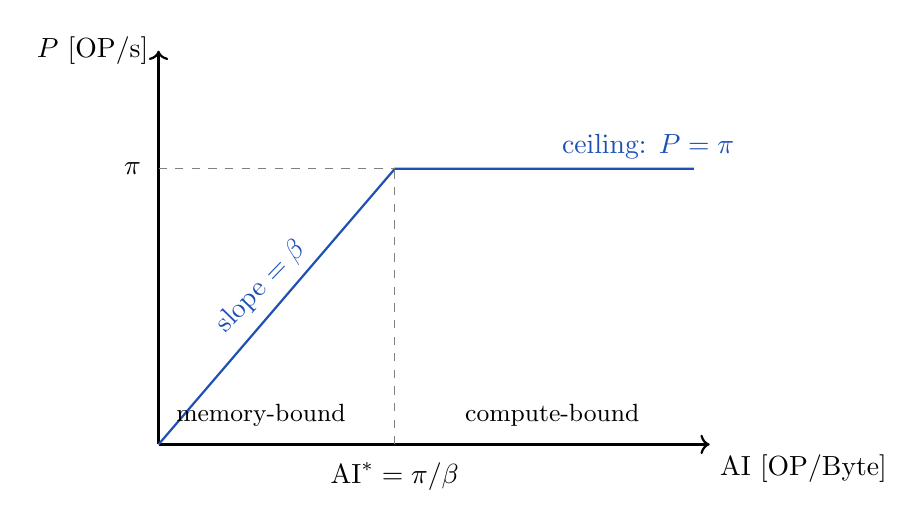
\begin{tikzpicture}[xscale=1.0, yscale=1.0]
    \draw[->, thick] (0,0) -- (7,0) node[below right] {$\AI\ [\mathrm{OP}/\mathrm{Byte}]$};
    \draw[->, thick] (0,0) -- (0,5) node[left] {$P\ [\mathrm{OP}/\mathrm{s}]$};
    \draw[thick, gpuColor] (0,0) -- (3,3.5) -- (6.8,3.5);
    \draw[dashed, gray] (3,0) -- (3,3.5);
    \draw[dashed, gray] (0,3.5) -- (3,3.5);
    \node[below] at (3,-0.1) {$\AI^{*} = \pi/\beta$};
    \node[left] at (-0.1,3.5) {$\pi$};
    \node[above right, gpuColor] at (5, 3.5) {ceiling: $P = \pi$};
    \node[rotate=46, gpuColor] at (1.3, 2.0) {slope $= \beta$};
    \node[above, align=center, font=\small] at (1.3, 0.1) {memory-bound};
    \node[above, align=center, font=\small] at (5.0, 0.1) {compute-bound};
\end{tikzpicture}
\caption{GPU Roofline 的几何结构。ceiling ($P=\pi$ 水平线) 与 slope ($P=\beta\cdot\AI$ 斜线) 交会于脊点 $\AI^{*}=\pi/\beta$，将平面划分为 memory-bound 与 compute-bound 两个区域。}
\label{fig:gpu_roofline}
\end{figure}

换言之，Roofline 本质上是在追问“任务的时空复杂度比例 vs 硬件的时空处理能力”的匹配度。

\subsection{三条架构前提：(P1)--(P3)}
\label{sec:gpu_premises}

公式~\eqref{eq:gpu_roofline} 的简洁形式来自三条隐含的架构前提，本文在第~\ref{sec:insight} 节将逐条审查这三条前提在 CIM 上是否仍成立：

\begin{description}[leftmargin=*, itemsep=2pt]
    \item[\textbf{(P1) 存算硬件分离}:] 计算单元与存储单元是两个独立的物理客体，各自拥有独立的速率指标($\pi$ 与 $\beta$)。
    \item[\textbf{(P2) 数据同类化}:] 所有进出计算单元的数据，在带宽层面无差别。权重、激活、中间变量统一以 Byte 计量、统一经由 memory channel。
    \item[\textbf{(P3) compute-memory 二元 $\max$ 归约}:] 性能瓶颈源自 compute 与 memory 两个物理独立资源的竞争；二者可流水线重叠，总时间下界取决于较慢者：$T \ge \max(T_{\mathrm{compute}},\ T_{\mathrm{move}})$。
\end{description}

(P1) 让两个硬件指标 $\pi$、$\beta$ 各自有可独立赋值的物理客体；(P2) 让所有数据通过同一个带宽通道而合并为单一 $\beta$;(P3) 让两个时间下界以 $\max$ 而非 $\sum$ 的方式归约，使 Roofline 几何呈现 “ceiling $+$ slope $+$ 脊点” 的标志性形态。三者共同支撑了“$P \le \min(\pi, \beta\cdot\AI)$”这一公式。三者共同呈现的“时间复杂度 vs 空间复杂度”分解，是冯诺依曼架构的\emph{物理印记}，并不是 Roofline 抽象本身的必然——这正是下一节的出发点。
\newpage

%% ===================================================================
\section{洞察：异构维度的反转}
\label{sec:insight}

本节展开三个步骤：CIM 系统性违反 (P1)--(P3)，三条违反背后是一个统一的\emph{结构反转}——异构维度从硬件转移到数据；由此 Roofline 的分解原则必须从“按硬件功能”改为“按操作数角色”；继而工作量的自然单位也从 OP 改为 Byte。这三步共同构成第~\ref{sec:cim_roofline} 节构建 CIM-native Roofline 的逻辑前提。

\subsection{CIM 对(P1)--(P3)的系统性违反：(A1)--(A3)}
\label{sec:violations}

将第~\ref{sec:gpu_premises} 节提出的三条前提逐条放到 CIM 上检验，得到三条对应的违反：

\begin{description}[leftmargin=*, itemsep=2pt]
    \item[\textbf{(A1) 存算融合}:] 阵列本身既是存储又是计算。\emph{MAC 不是“计算单元执行的独立动作”}，而是权重和输入共同到位后物理定律(欧姆定律 + 基尔霍夫电流定律)涌现的瞬时结果。没有独立的 “compute engine” 可以被单独赋予速率。
    \item[\textbf{(A2) 数据异类化}:] 进入阵列的数据严格分为两类：长期驻留于 cell 的\emph{权重}(resident)、随任务到来并穿过阵列的\emph{输入/输出}(streaming)。这两类数据走\emph{物理独立}的通路：resident 走编程/刷新通路，streaming 走 DAC--WL--BL--ADC 通路。它们在硬件层面不可混为单一 Byte。
    \item[\textbf{(A3) streaming-resident 二元 $\max$ 归约}:] CIM 的两个约束资源是 streaming 通路与 resident 通路，二者是\emph{物理独立}的路径、可流水线重叠，总时间下界由较慢通路决定：$T \ge \max(T_S, T_R)$。$\max$ 形式保留，但“两个竞争资源”的身份从 compute-memory 换成 streaming-resident。需要指出的是，CIM 的“流水线重叠”依赖\emph{多 macro 错峰调度}(一个 macro 在算、另一个在刷)而非单 macro 内部的时间复用——这是与 GPU 的本质机制差异，详见~\ref{sec:pipeline} 节。
\end{description}

三条违反表面互相独立，背后共享一个\emph{统一的结构反转}。

\subsection{异构维度反转与分解原则的转向}
\label{sec:inversion}

GPU 与 CIM 的本质区别不在“计算在哪”，也不在“数据如何搬”，而在于它们把\emph{异构性}放在了哪个维度上：

\begin{center}
\begin{tabular}{@{} l c c @{}}
\toprule
 & GPU(冯诺依曼) & CIM \\
\midrule
\textbf{硬件维度} & 异构(compute unit $\neq$ memory unit) & 同质(阵列处处都是 MAC) \\
\textbf{数据维度} & 同质(Byte 就是 Byte) & 异构(resident 权重 vs streaming 激活) \\
\bottomrule
\end{tabular}
\end{center}

\medskip
GPU 是“\textbf{异构硬件} $\times$ \textbf{同质数据}”；CIM 是“\textbf{同质硬件} $\times$ \textbf{异构数据}”。两者\emph{互为对偶}：把 GPU 的异构维度从硬件搬到数据，就得到 CIM。

这一反转直接决定了 Roofline 该如何分解任务量。在 GPU 上，$\pi$ 与 $\beta$ 之所以能作为两个正交的硬件指标，是因为对应的物理客体本身分离；“计算量”与“访存量”之所以能作为两个正交的模型指标，是因为任务量被自然分成“让 compute 单元做的事”与“让 memory 单元做的事”。在 CIM 上，硬件侧没有可分离的“两个客体”：阵列是一个整体物理装置。若强行沿用“算力 $+$ 带宽”的分法，会立即遇到两个无法解决的问题：CIM 的“算力”如何定义？MAC/s 不是独立动作，无法脱离数据路径独立赋值；CIM 的“带宽”如何定义？输入带宽、输出带宽、编程带宽几个量物理独立，无法合并为单一 $\beta$。

这两个问题不是命名层面的，而是“按硬件功能分解”在 CIM 上\emph{没有可分解的对象}。合理的处理是\emph{改换 CIM 下可分解的维度}，即操作数角色：
\begin{itemize}[topsep=2pt, itemsep=1pt]
    \item 经典 Roofline 按\textbf{硬件功能}分解任务量(哪部分归 compute，哪部分归 memory)，因为\emph{硬件是异构维度};
    \item CIM Roofline 应按\textbf{操作数角色}分解任务量(哪部分是 resident，哪部分是 streaming)，因为\emph{数据是异构维度}。
\end{itemize}

\subsection{工作量单位从 OP 转向 Byte}
\label{sec:work_unit}

伴随分解原则反转，一个更深的转变随之出现：\textbf{工作量的计量单位也必须改变}。

GPU 上 $\mathrm{OP}$ 之所以能作为 workload 的自然单位，是因为存在一个物理事实做支撑：\emph{每一个 OP 对应计算单元的一次独立硬件动作}。硬件“做了多少 OP”直接线性决定时间花销，所以用 OP 计量 workload 是恰当的。

CIM 上这一对应消失。MAC 不是“硬件执行的动作”，而是 resident 与 streaming 到位后由\emph{物理定律同时完成}的涌现结果。真正消耗时间的只有两件事：
\begin{enumerate}[topsep=2pt, itemsep=1pt]
    \item 把一份 streaming 数据通过 DAC--WL--阵列--BL--ADC 这条物理通路，消耗 streaming 通道容量；
    \item 把一份 resident 数据编程到阵列 cell，消耗 resident 通道容量。
\end{enumerate}
\emph{除此之外没有任何动作消耗时间。}MAC 从不单独消耗时间；它是前两件事发生时的同步结果。

因此，CIM 下 workload 的自然单位不是 OP，而是 \textbf{Byte}——具体而言是\emph{流过/写入通路的字节数}。Byte 既可作为 streaming 数据的总量 $Q_S$，也可作为 resident 数据的总量 $Q_R$，分别对应两类操作数在各自通路上的累计消耗。这与“按操作数角色分解”相一致：workload 总量被分解为 $(Q_S, Q_R)$ 两个 Byte 型量。$Q_S$、$Q_R$ 的形式定义、单位、与 $\RI$ 的引出在第~\ref{sec:cim_roofline} 节系统给出。
\newpage

%% ===================================================================
%% Phase 2 COMPLETED -- §4 CIM Roofline Model (5 subsections)
%% Phase 3 COMPLETED -- §5 quantitative calibration (4 subsections)
%% ---------------------------------------------------------------------
%% §4 has 5 subsections: indicators (window-based Q_R), formula/geometry,
%% pipeline mechanism, mode classification (with capacity and endurance
%% limits folded in), duality and coordinate transform (merged).
%%
%% §5 has 4 subsections: §5.1 parameter setup (table-based),
%%                       §5.2 hardware estimation (ρ for ACIM/DCIM,
%%                            τ for symmetric/asymmetric, FeNOR worked example),
%%                       §5.3 workload quantification (window-based, recomputed),
%%                       §5.4 2D regime matrix and discussion (folds in old §5.5).
%% Note: original §5.5 (robustness, engineering intuitions, design implications)
%%       distilled to a few paragraphs at the end of §5.4 per user request.
%% ===================================================================

\section{CIM Roofline 模型}
\label{sec:cim_roofline}

本节基于第~\ref{sec:insight} 节的洞察构建 CIM-native 的 Roofline。先在第~\ref{sec:cim_indicators} 节引入稳态分析窗口并在此窗口下定义两侧四指标与驻留强度, 继而在第~\ref{sec:cim_formula} 节给出公式与几何。第~\ref{sec:pipeline} 节与第~\ref{sec:modes} 节展开让公式工程可用所需的两件配套结构: pipeline 掩盖机制在 GPU 与 CIM 上的不同物理实现, 以及基于窗口的 workload 工况分类 (静态驻留与动态驻留, 含硬件容量与耐久度的额外限制讨论)。最后一节是存算分离与融合架构的对偶和转换 (第~\ref{sec:transform} 节), 含一张 GPU/CIM 系统对照表与以 workload 为中介的双向坐标变换。

\subsection{四个 CIM-native 指标: $\rho, \tau, Q_S, Q_R$ 与驻留强度 $\RI$}
\label{sec:cim_indicators}

按第~\ref{sec:inversion} 节的分解原则, CIM 的硬件侧与 workload 侧指标都按\emph{操作数角色}分解为 streaming 与 resident 两路: 硬件侧给出两条通路的吞吐率 $\rho$ 与 $\tau$; workload 侧给出两条通路上的累计字节 $Q_S$ 与 $Q_R$。$\RI$ 由这两对量的结构自然导出。

\paragraph{硬件侧: 流式数据吞吐 $\rho$ 与驻留数据吞吐 $\tau$}

\begin{definition}[流式数据吞吐 (Streaming throughput) $\rho$]
Streaming 通路每秒可稳定通过阵列的字节数, 单位 $[\mathrm{Byte}/\mathrm{s}]$。物理来源包括 DAC 转换、WL 驱动、阵列 settling、BL sensing、ADC 转换以及必要的后处理 (polling、mux、accumulation)。语义上 $\rho$ 刻画: \emph{一个已被编程好的 CIM 阵列在单位时间内能吞吐多少 streaming 操作数}。
\end{definition}

\begin{definition}[驻留数据吞吐 (Resident throughput) $\tau$]
Resident 通路每秒可稳定写入阵列的字节数, 单位 $[\mathrm{Byte}/\mathrm{s}]$。物理来源包括权重写入或编程通路的吞吐 (编程脉冲时间 $T_{\mathrm{prog}}$、并行编程单元数), 以及 endurance 约束下的平均可持续写入率。语义上 $\tau$ 刻画: \emph{CIM 每秒能把多少新权重加载到阵列, 使其进入可计算状态}。
\end{definition}

两指标\textbf{单位相同} (皆为 $\mathrm{Byte}/\mathrm{s}$)。这是一个结构性的信号: GPU 中 $\pi$ 与 $\beta$ 不同量纲, 因为 GPU 的两类硬件分别管辖\emph{时间}与\emph{空间}两个正交维度; 而 CIM 的两路通路管的都是同一物理类别, 即“数据通过通路的速率”, 故量纲一致。这从侧面印证, CIM 的对偶不是时-空对偶, 而是“两种数据通过通路”的对偶。

\paragraph{符号根源}
$\rho$ 取自希腊语 $\rho\acute{\epsilon}\omega$ (\emph{rheō}, 流动), 指 streaming 的物理意象; $\tau$ 取自希腊语 $\tau\acute{\alpha}\sigma\iota\varsigma$ (\emph{tasis}, 持拉或钉于其处), 指 resident 被驻定在阵列中的物理意象。两者都避开与 $\pi$、$\beta$ 同根, 以此强调 CIM 的两个硬件指标是\emph{全新的量}, 不是 GPU 指标的改写。

\paragraph{workload 侧的时间尺度: 稳态分析窗口}

硬件侧的 $\rho$ 与 $\tau$ 是纯硬件常数, 不依赖 workload 的时间形态。workload 侧的字节量则不然。Roofline 本质上是\emph{稳态吞吐}概念, 它回答的是“workload 在稳定工况下持续重复执行时每秒能达到多快”, 而不是“一次孤立事件的绝对耗时”。一次性的初始化事件 (如 workload 启动时把模型首次装载到阵列) 可被无限长的稳态摊销而不进入 Roofline 分析。由此, workload 侧的字节量必须绑定一个时间尺度, 即\emph{稳态分析窗口}。

\begin{definition}[稳态分析窗口 $W$]
workload 在稳定工况下的一个代表性重复单元, 刻画该工况每秒自我重复的基本模式。典型选取: 长期推理取“一次 forward”；LLM decode 取“一次 token 生成”；训练取“一次 step”；长会话取“一次 token 的 KV append”。$W$ 的绝对长度不进入任何比率型判据 (如 $\RI$ 与 $\RI^*$ 的比较), 它只为 workload 侧的两个字节量提供统一的时间坐标。
\end{definition}

\textbf{窗口内与窗口外的区分}。窗口外事件指 workload 生命周期内只发生有限次, 因此能被稳态无限摊销而逼近零开销的动作 (模型首次装载、一次性 warm-up、首 token 首次 pass 等); 窗口内事件指稳定运行中每周期都必然发生的动作。只有窗口内事件计入 $Q_S(W)$ 与 $Q_R(W)$, 窗口外事件不出现在 Roofline 分析中。

\begin{definition}[Streaming volume $Q_S(W)$]
窗口 $W$ 内经过 streaming 通路的字节总量, 单位 $[\mathrm{Byte}]$。对每 token 经过阵列的序列任务, $Q_S(W)$ 与序列长度、batch、层数、每窗口处理的 token 数线性相关。
\end{definition}

\begin{definition}[Resident volume $Q_R(W)$]
窗口 $W$ 内经过 resident 通路的字节总量, 单位 $[\mathrm{Byte}]$。由 workload 在窗口内是否触发写入决定:
\begin{itemize}[topsep=2pt, itemsep=1pt]
    \item 窗口内无权重或动态 resident 写入: $Q_R(W) = 0$。典型为模型已完成首次装载、处于稳态推理阶段。
    \item 窗口内有动态 resident 增长: $Q_R(W)$ 等于窗口内新写入阵列的字节, 典型为 attention 的 KV append。
    \item 窗口内有权重重写: $Q_R(W)$ 等于窗口内被重新编程的权重字节, 典型为 training step 或容量不足导致的权重重载。
\end{itemize}
\end{definition}

$Q_R(W)$ 的关键在于: 它是“窗口内通过 resident 通路的字节”, 不是“模型有多大”或“workload 累计写入多少字节”。一份 resident 字节只有在窗口内确实经过 $\tau$ 通路时才计入。这使 $Q_R$ 与 Roofline 公式里要除以 $\tau$ 的字节含义自动一致: 二者都是稳态下走 $\tau$ 通道的字节。对容量不足导致权重反复重装的情形, $Q_R(W)$ 自然包含这些反复装载所产生的额外流量, 详见第~\ref{sec:modes} 节关于硬件容量限制的讨论。

仿照 $\AI$ 的定义, 将 $Q_S(W)$ 与 $Q_R(W)$ 作比, 得到\textbf{驻留强度 (Resident Intensity)}:
\begin{equation}
\boxed{\;\RI(W) \;=\; \frac{Q_S(W)}{Q_R(W)}\quad [\text{dimensionless}].\;}
\label{eq:RI}
\end{equation}
约定: 当 $Q_R(W) = 0$ 时, $\RI(W) \to \infty$, 表示 workload 在窗口内完全不消耗 resident 通路。此时 Roofline 公式退化到 $P \le \rho$, $\tau$ 不进入瓶颈判断。

\textbf{符号约定}。后续章节中, $Q_S, Q_R, \RI$ 在不显式标注时均默认指给定稳态分析窗口 $W$ 下的值, 即 $Q_S(W), Q_R(W), \RI(W)$ 的简写。需要区分不同窗口或强调依赖关系时才写出 $(W)$。

\paragraph{算法语义}
$\RI$ 衡量\emph{每 Byte resident 数据支撑了多少 Byte 的 streaming 数据被处理}。这与 GPU 上 $\AI$ 衡量每搬运一份数据能承载多少计算的语义结构相同: $\AI$ 说的是数据搬到片上后被计算复用的密度, $\RI$ 说的是权重驻入阵列后被 streaming 复用的密度。形象地, resident 像一块驻定的海绵, streaming 像持续流过海绵的水: 高 $\RI$ 意味着同一块海绵被很多水浸透、复用充分; 低 $\RI$ 意味着海绵还没被充分浸透就要换新; $\RI = \infty$ 意味着窗口内根本不换海绵, resident 通路在稳态中完全空闲。

\paragraph{命名与量纲}
\begin{center}
\begin{tabular}{@{} l l l l @{}}
\toprule
\textbf{范式} & \textbf{强度} & \textbf{名字词根} & \textbf{词根含义} \\
\midrule
GPU & $\AI$ & \textbf{A}rithmetic & 强调“算术”, 即 GPU 以 compute 为第一阶事件 \\
CIM & $\RI$ & \textbf{R}esident & 强调“驻留”, 即 CIM 以 residency 为第一阶事件 \\
\bottomrule
\end{tabular}
\end{center}

每个范式的驻留强度名称都指向该范式的“核心”。$\AI$ 的量纲是 $\mathrm{OP}/\mathrm{Byte}$ (跨量纲比), $\RI$ 的量纲是 $\mathrm{Byte}/\mathrm{Byte}$ (无量纲纯比例): 前者反映 GPU 把任务分摊到\emph{异质硬件}, 后者反映 CIM 把任务分摊到\emph{异质数据}。

\subsection{公式与几何}
\label{sec:cim_formula}

\paragraph{公式推导}
对给定稳态分析窗口 $W$ 下的 workload:
\begin{align}
T_S &\ge Q_S/\rho \quad (\text{streaming 通路的时间下界}),\\
T_R &\ge Q_R/\tau \quad (\text{resident 通路的时间下界}).
\end{align}
由第~\ref{sec:violations} 节 (A3), streaming 与 resident 通路\emph{物理独立}且可\emph{流水线并行}, 总时间由较慢的通路决定:
\begin{equation}
T \;\ge\; \max\!\left(\frac{Q_S}{\rho},\ \frac{Q_R}{\tau}\right).
\end{equation}
CIM 的 workload 以 streaming 吞吐计量 (见第~\ref{sec:work_unit} 节): $P = Q_S/T\ [\mathrm{Byte}/\mathrm{s}]$。代入并利用 $\RI = Q_S/Q_R$ 得:
\begin{equation}
\boxed{\;P \;\le\; \min\!\bigl(\rho,\ \tau\cdot\RI\bigr)\quad [\mathrm{Byte}/\mathrm{s}].\;}
\label{eq:cim_roofline}
\end{equation}
这就是 CIM Roofline 公式。其形式与 GPU Roofline~\eqref{eq:gpu_roofline} 完全\emph{同构} (两者均取 $P \le \min(\text{ceiling},\ \text{slope} \times \text{intensity})$ 的形式), 但每一项的物理含义独立。

\paragraph{几何}
在以 $\RI$ 为横轴、$P$ 为纵轴的平面上 (图~\ref{fig:cim_roofline}), 公式~\eqref{eq:cim_roofline} 的 ceiling ($P = \rho$ 水平线, 对应流式吞吐受限区) 与 slope ($P = \tau \cdot \RI$ 斜线, 对应驻留吞吐受限区) 交于脊点 $\RI^{*} = \rho/\tau$ (纯硬件常数、无量纲)。

\begin{figure}[htbp]
\centering
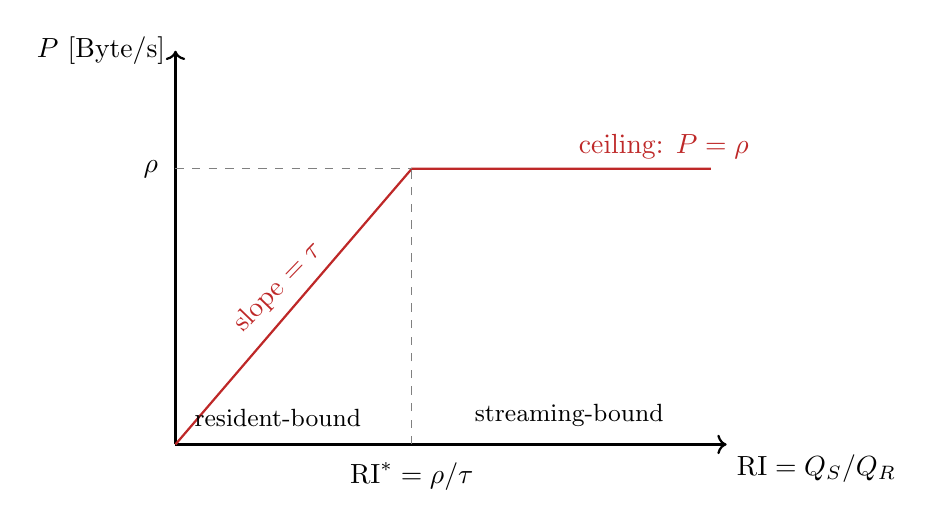
\begin{tikzpicture}[xscale=1.0, yscale=1.0]
    \draw[->, thick] (0,0) -- (7,0) node[below right] {$\RI = Q_S/Q_R$};
    \draw[->, thick] (0,0) -- (0,5) node[left] {$P\ [\mathrm{Byte}/\mathrm{s}]$};
    \draw[thick, cimColor] (0,0) -- (3,3.5) -- (6.8,3.5);
    \draw[dashed, gray] (3,0) -- (3,3.5);
    \draw[dashed, gray] (0,3.5) -- (3,3.5);
    \node[below] at (3,-0.1) {$\RI^{*} = \rho/\tau$};
    \node[left] at (-0.1,3.5) {$\rho$};
    \node[above right, cimColor] at (5, 3.5) {ceiling: $P = \rho$};
    \node[rotate=46, cimColor] at (1.3, 2.0) {slope $= \tau$};
    \node[above, align=center, font=\small] at (1.3, 0.1) {resident-bound};
    \node[above, align=center, font=\small] at (5.0, 0.1) {streaming-bound};
\end{tikzpicture}
\caption{CIM Roofline 的几何结构。ceiling ($P = \rho$ 水平线) 与 slope ($P = \tau\cdot\RI$ 斜线) 交会于脊点 $\RI^{*}=\rho/\tau$, 将平面划分为驻留吞吐受限 (resident-bound) 与流式吞吐受限 (streaming-bound) 两个区域。与图~\ref{fig:gpu_roofline} 的 GPU Roofline 形式同构, 但每条轴的物理语义独立定义。}
\label{fig:cim_roofline}
\end{figure}

\paragraph{受限分区语义}
\begin{description}[leftmargin=*, itemsep=2pt]
    \item[\textbf{驻留吞吐受限区 (resident-bound)} ($\RI < \RI^*$):] 算法 $\RI$ 过低, 使 $\tau \cdot \RI < \rho$; 每份权重只服务了很少 streaming 就要被换掉, resident 通路首先吃满。工程优化方向为\emph{抬高 $\RI$}, 即增大 batch、加长 prefill 序列、复用权重、缩减 expert 切换频率, 使每份驻留状态被更多 streaming 所复用。
    \item[\textbf{流式吞吐受限区 (streaming-bound)} ($\RI > \RI^*$):] 算法 $\RI$ 充分, 使 $\tau \cdot \RI > \rho$; resident 已被充分复用, streaming 通路首先吃满。工程优化方向为\emph{抬高硬件 $\rho$}, 即升级 ADC/DAC、增加接口并行度、压缩通路延时。
\end{description}

\paragraph{退化情形: $Q_R = 0$}
当窗口 $W$ 内不触发任何 resident 通路消耗时, $Q_R = 0$, $\RI \to \infty$, 公式~\eqref{eq:cim_roofline} 的 $\tau \cdot \RI$ 斜线退化为 $+\infty$, Roofline 简化为 $P \le \rho$: 性能仅由 $\rho$ 决定, $\tau$ 不进入瓶颈判断。这对应\emph{窗口内无写入的稳态工况}, 例如模型已装载完毕、长期推理的静态部署场景。

\subsection{Pipeline 机制: GPU 与 CIM 的物理实现差异}
\label{sec:pipeline}

公式~\eqref{eq:cim_roofline} 由 $T \ge \max(T_S, T_R)$ 推得。$\max$ 归约背后的物理前提是 streaming 与 resident 两条通路可流水线重叠。这一前提在 GPU 与 CIM 上由不同物理机制实现, 必须分别说明。

\paragraph{GPU: 时间复用}
同一份 compute unit 在第 $N$ 轮做 MAC 的同时, 同一份 memory channel 在搬第 $N+1$ 轮的数据。两个独立硬件客体在\emph{时间维度}上交错执行, 掩盖天然成立。

\paragraph{CIM: 空间复用}
同一个 CIM macro 物理上不能同时编程 cell 又读电流做 MAC, 两种动作竞争同一阵列资源。掩盖必须依赖多 macro 或多 bank 协作: macro $A$ 在做 streaming MAC 的同时, macro $B$ 在被编程刷新; 下一轮交换。这是\emph{空间维度}上的错峰。

\paragraph{对硬件的隐含要求}
形式上 $\max$ 归约对称, Roofline 几何不变。但 CIM 的 $\max$ 归约隐含一个额外的硬件前提: 有足够多的 macro 可以错峰调度。若硬件只有单 macro, resident 与 streaming 通路无法重叠, $\max$ 退化为 $\sum$, 实际性能落在 Roofline 上界之下。CIM Roofline 的“理想性能上界”对应 macro 数量充分时的稳态。

\paragraph{“被掩盖” 的语义}
驻留吞吐受限或流式吞吐受限并不意味着另一条通路闲置, 只意味着另一条通路的时间被掩盖了。流式吞吐受限区中 resident 通路仍在持续工作, 只是 $T_R < T_S$, 故其时间不显形于总时间; 反之亦然。被掩盖的通道仍持续消耗硬件资源 (带宽、功耗、endurance), 只是不影响吞吐。

\subsection{工况分类: 静态驻留与动态驻留}
\label{sec:modes}

\paragraph{Resident 更新率}
基于第~\ref{sec:cim_indicators} 节定义的 $Q_R(W)$, 可以引出一个 workload 属性的派生量:
\begin{equation}
\frac{\mathrm{d}Q_R}{\mathrm{d}t} \;\equiv\; \frac{Q_R(W)}{|W|} \quad [\mathrm{Byte}/\mathrm{s}],
\end{equation}
即 workload 在稳态下每秒经 resident 通路写入阵列的字节数, 称为\textbf{Resident 更新率}。这是 workload 属性, 不是硬件属性, 不进入 Roofline 公式。它与硬件 $\tau$ 的比较决定了 $\tau$ 在稳态下是否成为真实瓶颈。

\paragraph{二分: 静态驻留与动态驻留}
按 $\mathrm{d}Q_R/\mathrm{d}t$ 的稳态值 (等价地, 按 $Q_R(W)$ 是否为零), CIM workload 落入两类本质不同的工况。

\begin{description}[leftmargin=*, itemsep=2pt]
    \item[\textbf{静态驻留}, $\mathrm{d}Q_R/\mathrm{d}t = 0$:] 稳态窗口内不触发 resident 通路写入。此时 $\RI \to \infty$, Roofline 退化为 $P \le \rho$, $\tau$ 不进入瓶颈判断。典型场景是模型一次烧入即长期推理。
    \item[\textbf{动态驻留}, $\mathrm{d}Q_R/\mathrm{d}t > 0$:] 稳态窗口内有 resident 通路写入, $\tau$ 以真实 bottleneck 成员身份显形于公式, regime 由 $\RI$ 与 $\RI^*$ 的比较决定。
\end{description}

动态驻留内部按 $\mathrm{d}Q_R/\mathrm{d}t$ 的量级可进一步分为缓慢累积 (例如 KV append) 与持续重写 (例如 training step 或权重换页) 两种叙述类别。这一细分不进入 Roofline 判据, 仅服务叙述。Roofline 公式只关心 $Q_R(W) = 0$ 是否成立。

\paragraph{硬件容量的限制}
工况虽是 workload 属性, 但硬件容量可以反过来推动 workload 在两类工况之间迁移。三种代表性情形:

\begin{itemize}[topsep=2pt, itemsep=4pt]
    \item \textbf{大容量阵列 + 中小模型推理}: 模型一次装入即可服役全 workload, 自然落入静态驻留。即使硬件 $\tau$ 物理上很低, 稳态吞吐也不受其拖累。这是 NOR Flash CIM 这类 $\tau$ 极低、容量极大的技术能承担静态推理的根源。
    \item \textbf{小容量阵列 + 大模型推理}: 模型不能一次装入, 执行中必须分块反复重新编程。workload 名义上是推理 (本应静态驻留), 实际上被强制进入持续重写, $\mathrm{d}Q_R/\mathrm{d}t$ 显著大于零。$\tau$ 是否构成瓶颈由其与 streaming 需求频率 $\rho \cdot \RI$ 的关系决定。SRAM-CIM 类 $\tau$ 较高但容量极小的技术在大模型场景下出现 resident 瓶颈, 根源就在容量限制本身, 而不是 $\tau$ 不够。
    \item \textbf{训练}: 不论硬件容量大小, 每个 backward step 都必须将更新后的权重回写阵列, workload 内禀属于持续重写, $\mathrm{d}Q_R/\mathrm{d}t$ 与 step 频率成正比。$\tau$ 是否构成瓶颈仍由 $\RI$ 与 $\RI^*$ 的比较决定, 并不必然落入驻留吞吐受限区。
\end{itemize}

\paragraph{硬件耐久性的限制}
除了容量, CIM 器件在时间维度上还有一类与硬件相关的限制: 写循环数有限的非易失器件 (例如 RRAM、Flash) 在长时间持续 resident 通路写入下, 可持续的 $\mathrm{d}Q_R/\mathrm{d}t$ 受器件寿命约束。即使瞬时 $\tau$ 较高, 长期摊销下的有效 $\tau$ 也会被压低。SRAM、FeFET 等高循环耐久度器件不受此限; RRAM、NAND 等低耐久度器件在动态驻留 workload 下需要把这一项纳入考量。容量限制与耐久度限制描述不同维度的硬件约束, 不能合并: 前者按每次窗口的写入字节计入, 后者按累计写入次数的器件上限计入。

\paragraph{小结}
Roofline 公式 $P \le \min(\rho, \tau \cdot \RI)$ 对所有工况形式不变。$\tau$ 是否进入瓶颈完全由窗口内 resident 通路是否被触发决定: $Q_R(W) = 0$ 时退化为 $P \le \rho$; $Q_R(W) > 0$ 时由 $\RI$ 与 $\RI^*$ 的比较决定 regime。硬件容量与耐久度则在公式之外约束实际可达的工作点: 容量限制可以把名义为静态驻留的 workload 推入动态驻留, 耐久度则压低长时摊销下的有效 $\tau$。这两点在 CIM 工程分析中容易被遗漏。

\subsection{存算分离和融合架构的对偶和转换}
\label{sec:transform}
\label{sec:comparison}

GPU 与 CIM 在第~\ref{sec:inversion} 节意义下互为对偶: 一个把硬件分裂、数据同质化, 一个把硬件同质化、数据分裂。这种对偶在 Roofline 层面有两个具体表现, 本节合并讨论。先用一张对照表把两套 Roofline 的指标、公式、几何摆在一起, 看出它们形式同构、语义独立的对应关系; 然后给出以 workload 为中介的双向坐标变换, 把工程上常说的 “CIM macro 算力 X TOPS” 这种语言还原到本框架的指标体系里。

\begin{table}[h!]
\centering
\small
\renewcommand{\arraystretch}{1.25}
\begin{tabular}{@{} p{0.24\textwidth} p{0.34\textwidth} p{0.34\textwidth} @{}}
\toprule
\textbf{维度} & \textbf{GPU Roofline} & \textbf{CIM Roofline} \\
\midrule
任务量分解原则 & 按\emph{硬件功能} & 按\emph{操作数角色} \\
算法任务量 A & OP (compute 单元承担) & $Q_S$ (streaming 通路字节, 窗口内) \\
算法任务量 B & Byte (memory 通道承担) & $Q_R$ (resident 通路字节, 窗口内) \\
\midrule
硬件速率 A & $\pi\ [\mathrm{OP}/\mathrm{s}]$ (算力) & $\rho\ [\mathrm{Byte}/\mathrm{s}]$ (流式数据吞吐) \\
硬件速率 B & $\beta\ [\mathrm{Byte}/\mathrm{s}]$ (带宽) & $\tau\ [\mathrm{Byte}/\mathrm{s}]$ (驻留数据吞吐) \\
\midrule
驻留强度 & $\AI = \mathrm{OP}/\mathrm{Byte}$ & $\RI = Q_S/Q_R$ \\
强度名字词根 & \textbf{A}rithmetic (GPU 核心) & \textbf{R}esident (CIM 核心) \\
强度量纲 & $\mathrm{OP}/\mathrm{Byte}$ (跨量纲比) & 无量纲 (同量纲比) \\
\midrule
性能 Y 轴单位 & $\mathrm{OP}/\mathrm{s}$ & $\mathrm{Byte}/\mathrm{s}$ \\
Roofline 公式 & $P \le \min(\pi,\ \beta\cdot\AI)$ & $P \le \min(\rho,\ \tau\cdot\RI)$ \\
Y 轴语义 & 时间复杂度吞吐 & 流动复杂度吞吐 \\
X 轴语义 & 时间复杂度 / 空间复杂度 & 流动复杂度 / 驻留复杂度 \\
斜率语义 & 搬运带宽 (空间/时间) & 更换吞吐 (驻留/时间) \\
\midrule
左侧受限区 & memory-bound (存储受限) & 驻留吞吐受限 (resident-bound) \\
右侧受限区 & compute-bound (算力受限) & 流式吞吐受限 (streaming-bound) \\
脊点 & $\AI^{*} = \pi/\beta\ [\mathrm{OP}/\mathrm{Byte}]$ & $\RI^{*} = \rho/\tau\ [\text{无量纲}]$ \\
\bottomrule
\end{tabular}
\caption{GPU Roofline 与 CIM Roofline 的系统性对偶。两者形式同构而语义独立, 每一行的左右两列分别是各自架构下的对应量。}
\label{tab:comparison}
\end{table}

\paragraph{出发的问题}
GPU 的算力 $\pi$ 与带宽 $\beta$ 之所以能脱离 workload 而存在, 物理依据来自第~\ref{sec:gpu_premises} 节的两条架构前提: 计算单元与存储单元各自是独立硬件客体, 所以 $\pi$、$\beta$ 各自有可独立赋值的速率 (P1); 数据被同质化为 Byte, 每个 OP 都对应 compute unit 的一次独立动作, 与 OP 来自权重侧还是激活侧无关 (P2)。两条合起来使 OP/s 与 Byte/s 这两个数字脱离 workload 仍有意义。CIM 同时违反这两条 (第~\ref{sec:violations} 节 (A1) 与 (A2)), 自然失去这种 “硬件指标可独立赋值” 的基础。但工程上 CIM macro 仍然按惯例报 “算力 X TOPS”。本节回答两个问题: 这个数字到底是什么? 同一 workload 在 GPU 与 CIM 两套 Roofline 坐标系里如何相互换算?

\paragraph{Workload 的三元描述与结构常数 $\kappa_S, \kappa_R$}
\label{para:kappa_def}
一个 workload 由三个独立的基本量完整刻画: 总 MAC 数 $M\ [\mathrm{OP}]$, streaming 通路字节 $Q_S\ [\mathrm{Byte}]$, resident 通路字节 $Q_R\ [\mathrm{Byte}]$ (后两者按第~\ref{sec:cim_indicators} 节的窗口定义)。GPU Roofline 用二元投影 $(M,\ Q_S+Q_R)$ 分解任务, CIM Roofline 用二元投影 $(Q_S,\ Q_R)$ 分解任务。两者是同一个三元组在不同坐标轴下的两个切面。

跨切面的换算需要中介量。定义两个 workload 结构常数:
\begin{equation}
\kappa_S \;=\; \frac{M}{Q_S}\ \ [\mathrm{OP}/\mathrm{Byte}], \qquad
\kappa_R \;=\; \frac{M}{Q_R}\ \ [\mathrm{OP}/\mathrm{Byte}],
\end{equation}
分别衡量 “每字节 streaming 数据承载多少个 MAC” 与 “每字节 resident 数据参与多少个 MAC”。两者只由算法或模型结构决定, 与执行硬件无关。在静态驻留下 $Q_R = 0$, $\kappa_R$ 不定义, 这与 $\RI \to \infty$ 的边界情形一致。

由 $\kappa_S Q_S = \kappa_R Q_R = M$ 立即得:
\begin{equation}
\boxed{\ \RI \;=\; \frac{Q_S}{Q_R} \;=\; \frac{\kappa_R}{\kappa_S}.\ }
\label{eq:RI_kappa}
\end{equation}
$\RI$ 由此获得第二重语义: 同一 workload 在 streaming 侧与 resident 侧的 “计算密度” 之比。对稠密线性层 ($W \in \mathbb{R}^{N \times M_w}$, batch $B$, 每元素 $b$ 字节): $M = BNM_w$, $Q_R = NM_w b$, $Q_S = BM_w b$, 代入得 $\kappa_R = B/b$, $\kappa_S = N/b$。可见 $\kappa_S$ 中的 batch 因子被 $Q_S$ 中的 batch 因子抵消, 因此 $\kappa_S$ 与 batch 大小无关, 只取决于模型结构 $N$ 与精度 $b$。

\paragraph{算例: 28\,nm SRAM ACIM macro}
设阵列 $N \times N = 128 \times 128$, INT8 cell (每权重 1 字节), cycle time $T = 10$\,ns。一次 MVM 中, 经 streaming 通路的字节数为 $N = 128$, 涉及的 MAC 操作数为 $N^2 = 16{,}384$ (按每个 MAC 算 2 OP, 共 $2N^2 = 32{,}768$ OP), 权重已驻留阵列中、本次不经 resident 通路, 每秒可跑 $1/T = 10^8$ 次 MVM。

由这些数直接给出本节定义的 streaming 通路吞吐 $\rho$ 与 CIM macro 上常报的算力:
\[
\rho \;=\; \frac{128\,\mathrm{B}}{10\,\mathrm{ns}} \;=\; 12.8\,\mathrm{GB/s}, \qquad
\pi \;=\; \frac{32{,}768\,\mathrm{OP}}{10\,\mathrm{ns}} \;=\; 3.28\,\mathrm{TOPS}.
\]

观察这两个数: 算力 $\pi$ 除以 streaming 吞吐 $\rho$ 得到 $3.28\,\mathrm{TOPS} \div 12.8\,\mathrm{GB/s} = 256\,\mathrm{OP/Byte}$, 是一个不依赖时间单位的纯结构常数。这并非巧合: 它正好等于这次 MVM 中总 OP 数与 streaming 字节数的比 $32{,}768 / 128 = 2N$。也就是说,
\[
\pi \;=\; 2N \times \rho.
\]

这个 $2N$ 系数完全由 MVM 的算法结构 (阵列宽度 $N$) 决定, 与硬件时钟、阵列工艺都无关。它衡量 “每字节 streaming 数据承载多少个 MAC”, 正是上文定义的 workload 结构常数 $\kappa_S = M/Q_S$。两边因而可以写成更一般的形式:
\begin{equation}
\pi \;=\; \kappa_S \times \rho.
\label{eq:tops_demystify}
\end{equation}
这样, “CIM macro 算力” 就被还原成了一种投影量: 它是 $\rho$ 通过 workload 结构常数 $\kappa_S$ 投影到 OP/s 坐标后的结果, 而不是脱离 workload 单独存在的硬件指标。同一片 CIM macro 在不同 workload 下报出的 “算力” 可能差几个数量级, 这并不是芯片性能在变, 而是 $\kappa_S$ 这个投影系数随 workload 在变。

\paragraph{等效算力 $\pi_{\mathrm{eq}}$ 与等效带宽 $\beta_{\mathrm{eq}}$: 把 CIM 投到 GPU 坐标}
算例只考虑了 streaming 通路。一般情况下若 resident 通路也消耗时间 (动态驻留), 等效算力是两条通路通过 $\kappa$ 投影后取较小者:
\begin{equation}
\boxed{\ \pi_{\mathrm{eq}}(W) \;=\; \min\!\bigl(\kappa_S \rho,\ \kappa_R \tau\bigr) \quad [\mathrm{OP}/\mathrm{s}].\ }
\label{eq:pi_eq}
\end{equation}
CIM macro 上常报的 “X TOPS” 对应 $\max_W \pi_{\mathrm{eq}}(W)$, 即一个理想 workload (典型为满阵列 MVM 且无 resident reload) 下的上界。真实 LLM workload 下能取得的性能可能远低于这一上界。

与等效算力对偶, 还存在一个等效带宽。把整个 CIM 视作一个 “数据吞吐口”, 外部观察者看到的合成流速为:
\begin{equation}
\boxed{\ \beta_{\mathrm{eq}}(W) \;=\; \frac{Q_S + Q_R}{\max(Q_S/\rho,\ Q_R/\tau)} \quad [\mathrm{Byte}/\mathrm{s}].\ }
\label{eq:beta_eq}
\end{equation}
几何上, 这是把 CIM 两条独立物理通路在 pipeline 重叠下压成一条等效单管道, 流速即 $\beta_{\mathrm{eq}}$。在静态驻留下 ($Q_R = 0$) $\beta_{\mathrm{eq}}$ 退化为 $\rho$。工程上常常只谈 CIM 的等效算力, 不谈等效带宽。原因在于大家用 GPU 视角看 CIM 时, 看到 CIM 把权重驻留在阵列里、激活直接流过阵列做计算, 觉得 CIM 已经把 “访存” 这个老问题彻底解决了, 自然认为 “带宽” 这个概念在 CIM 上不再需要, 只剩下 “算力” 一项。但实际上 CIM 仍有真实的字节通过物理通路, 这些字节经过 pipeline 重叠后给出的合成流速就是等效带宽。它与等效算力同样存在, 同样依赖 workload, 只有把两者并列, 才能与 GPU 的 $(\pi, \beta)$ 二元指标真正完整对照。

\paragraph{反向投影 $\rho_{\mathrm{eq}}, \tau_{\mathrm{eq}}$: 把 GPU 投到 CIM 坐标}
\label{para:bidirectional}
对称地, GPU 在 CIM 坐标下也有等效流动与等效驻留。给定 GPU 硬件 $(\pi, \beta)$ 与具体 workload, GPU 完成该 workload 的实际时间下界为:
\[
T_{\mathrm{GPU}} \;=\; \max\!\bigl(M/\pi,\ (Q_S+Q_R)/\beta\bigr).
\]
则:
\begin{align}
\rho_{\mathrm{eq}}(W) &\;=\; \frac{Q_S}{T_{\mathrm{GPU}}} \quad [\mathrm{Byte}/\mathrm{s}], \label{eq:rho_eq} \\
\tau_{\mathrm{eq}}(W) &\;=\; \frac{Q_R}{T_{\mathrm{GPU}}} \quad [\mathrm{Byte}/\mathrm{s}]. \label{eq:tau_eq}
\end{align}
物理含义: 把 GPU 视作对该 workload 同时流过 $Q_S$ 字节、写入 $Q_R$ 字节的等效系统 (尽管 GPU 内部根本不区分两者), 等效流动率与等效驻留率分别由分子定义、分母即 GPU 完成 workload 的实际时间。这两个量与 $\pi_{\mathrm{eq}}, \beta_{\mathrm{eq}}$ 完全对称。

\paragraph{双向变换对照}
\begin{center}
\small
\renewcommand{\arraystretch}{1.25}
\begin{tabular}{@{} l l l @{}}
\toprule
\textbf{投影方向} & \textbf{目标坐标系} & \textbf{等效硬件指标} \\
\midrule
CIM $(\rho,\tau) \to$ GPU 坐标 & $(\pi, \beta)$ & $\pi_{\mathrm{eq}} = \min(\kappa_S\rho,\ \kappa_R\tau);\quad \beta_{\mathrm{eq}} = (Q_S+Q_R)/T_{\mathrm{CIM}}$ \\
GPU $(\pi,\beta) \to$ CIM 坐标 & $(\rho, \tau)$ & $\rho_{\mathrm{eq}} = Q_S/T_{\mathrm{GPU}};\quad \tau_{\mathrm{eq}} = Q_R/T_{\mathrm{GPU}}$ \\
\bottomrule
\end{tabular}
\end{center}

其中 $T_{\mathrm{CIM}} = \max(Q_S/\rho,\ Q_R/\tau)$、$T_{\mathrm{GPU}} = \max(M/\pi,\ (Q_S+Q_R)/\beta)$。注意 “GPU 算力 X TFLOPS” 与 “CIM macro 算力 X TOPS” 两种说法表面相似但语义层级不同: 前者是硬件常数 $\pi$ 本身, 后者是 $\pi_{\mathrm{eq}}$ 的 max projection。

\paragraph{Y 轴与 X 轴的显式变换}
\label{para:axis_xform}
作为副产品, 同一 workload 在两套 Roofline 平面上的坐标也可以直接换算。Y 轴: $P_{\mathrm{GPU}} = M/T$, $P_{\mathrm{CIM}} = Q_S/T$, 由 $M = \kappa_S Q_S$ 得 $P_{\mathrm{GPU}} = \kappa_S \cdot P_{\mathrm{CIM}}$, 转换系数是 workload 属性而非硬件常数。X 轴: $\AI$ 与 $\RI$ 的关系是
\begin{equation}
\AI \;=\; \frac{M}{Q_S+Q_R} \;=\; \frac{\kappa_S Q_S}{Q_S+Q_R} \;=\; \kappa_S \cdot \frac{\RI}{\RI + 1},
\label{eq:AI_RI}
\end{equation}
是以 $\kappa_S$ 为参数的分数线性变换, 不是简单线性比例。两个极限: $\RI \to \infty$ 时 $\AI \to \kappa_S$; $\RI \to 0$ 时 $\AI \to 0$。

\paragraph{不对称的根源}
上面四个等效量都依赖具体 workload, 而 GPU 自身的 $(\pi, \beta)$ 与 CIM 自身的 $(\rho, \tau)$ 都与 workload 无关。这一不对称看似奇怪, 其实有清楚的物理来源。每种架构在自己原生的坐标系里, 硬件指标与 workload 指标是按同一个维度分解的: GPU 把硬件分解成计算单元和存储单元, 也把 workload 分解成计算量 (OP) 和访存量 (Byte), 两套分解在 “功能” 维度上一一对应, 因此 $(\pi, \beta)$ 在 GPU 坐标里就是纯硬件常数; CIM 把硬件分解成 streaming 通路与 resident 通路, 也把 workload 分解成流过的字节与驻留的字节, 两套分解在 “角色” 维度上一一对应, 因此 $(\rho, \tau)$ 在 CIM 坐标里同样是纯硬件常数。

跨架构投影时, 这种自然对齐就被打破了。要把 “按角色分的” 映到 “按功能分的”, 必须知道每一个 MAC 对应的字节属于哪一类角色, 而这个信息只能由 workload 提供, 硬件本身无法预先回答。$\kappa_S$ 与 $\kappa_R$ 就是这个信息的形式化, 也正因为如此, 经它们投影出来的等效硬件指标必然带 workload 标签。可以这样理解: “硬件指标是不是常数” 这个问题本身依赖于坐标系。在某个架构原生的坐标系里它是常数, 跨到另一架构的坐标系里就成了 workload 的函数。这跟物理学里 “是否同时” 依赖于参考系是同一种结构性事实, 不是框架的缺陷。

\paragraph{小结}
两套 Roofline 系统不能在纯硬件层面互相映射, 因为 OP 与 Byte 是不同物理量, 之间的 “汇率” $\kappa$ 必然由 workload 决定。但在 $\kappa_S, \kappa_R$ 引入之后, 跨坐标变换是双向、完整、对称的: CIM 投到 GPU 得到 $\pi_{\mathrm{eq}}, \beta_{\mathrm{eq}}$; GPU 投到 CIM 得到 $\rho_{\mathrm{eq}}, \tau_{\mathrm{eq}}$。CIM macro 上常报的 “算力 X TOPS” 在本框架里被还原为 $\pi_{\mathrm{eq}}$ 的 max projection: 它不是错误也不绝对, 只是某一坐标系下的一种描述。
\newpage

%% ===================================================================
\section{硬件与 workload 的定量标定}
\label{sec:quantitative}

第~\ref{sec:cim_roofline} 节给出了 CIM Roofline 的形式化定义。本节把硬件指标 ($\rho$, $\tau$) 与 workload 指标 ($Q_S$, $Q_R$, $\RI$) 按解析方式算清, 并把硬件 $\times$ workload 的两维结果汇成 regime 矩阵。先在第~\ref{sec:assumptions} 节作参数前置, 再分别标定硬件 (第~\ref{sec:hw_quant} 节) 与 workload (第~\ref{sec:wl_quant} 节), 最后在第~\ref{sec:matrix_eval} 节做二维 regime 分析并讨论对器件与算法设计的启示。

\subsection{估算框架与参数前置}
\label{sec:assumptions}

本节把后续硬件指标估算所需的全部参数一次列清, 并给出器件层面与任务层面的基线取值, 后文公式只在表上代数。所有讨论限定在 28\,nm CMOS 外围电路基线下, 以便不同 cell 技术之间做公平对比: 不同 cell 技术的 backend 与堆叠形态可独立演化, 但 DAC、ADC、字线驱动、位线 sensing 等 CMOS 外围电路在该基线下近似等价。

\paragraph{硬件通用参数}
两条通路所用的延时与并行度参数列于表~\ref{tab:hw_params}。其中两个量 ($T_{\mathrm{cell}}$ 与 $T_{\mathrm{prog}}$) 对器件技术高度敏感, 单独列于表~\ref{tab:cell_params}, 跨器件可差几个数量级。

\begin{table}[h!]
\centering
\small
\renewcommand{\arraystretch}{1.2}
\begin{tabular}{@{} l p{0.32\textwidth} l l p{0.22\textwidth} @{}}
\toprule
\textbf{符号} & \textbf{物理含义} & \textbf{基线} & \textbf{范围} & \textbf{备注} \\
\midrule
$T_{\mathrm{DAC}}$ & DAC 转换时延 & 1\,ns & 0.5--3\,ns & 4-bit 电阻分压式即可 \\
$T_{\mathrm{WL}}$ & 字线驱动 (含 RC 寄生) & 2\,ns & 1--5\,ns & 依字线长度与走线 \\
$T_{\mathrm{cell}}$ & cell 读响应 & \multicolumn{2}{l}{见表~\ref{tab:cell_params}} & 跨器件差几个数量级 \\
$T_{\mathrm{BL}}$ & 位线 settling & 3\,ns & 2--10\,ns & 依 BL 电容与驱动电流 \\
$T_{\mathrm{ADC}}$ & 8-bit SAR ADC 单次转换 (ACIM) & 8\,ns & 5--15\,ns & ACIM 关键瓶颈 \\
$T_{\mathrm{AT}}$ & adder tree 组合延时 (DCIM) & 3\,ns & 2--5\,ns & 替代 $T_{\mathrm{ADC}}$ \\
$T_{\mathrm{prog}}$ & 单次编程脉冲 & \multicolumn{2}{l}{见表~\ref{tab:cell_params}} & 跨器件差几个数量级 \\
$T_{\mathrm{erase}}$ & 单次擦除 & 对称 cell: $=T_{\mathrm{prog}}$ & — & NAND: $\sim$15\,ms/block \\
$k_{\mathrm{verify}}$ & 平均 verify-retry 次数 & \multicolumn{2}{l}{见表~\ref{tab:cell_params}} & NVM 类必需 \\
$N_{\mathrm{par\text{-}write}}$ & 单脉冲并行写入 cell 数 & 128 & 64--512 & 受字线驱动能力限制 \\
$N_{\mathrm{bank}}$ & macro 内并行 bank 数 & 4 & 2--16 & 设计选择 \\
\bottomrule
\end{tabular}
\caption{硬件通用参数。所有时延均为 28\,nm CMOS 外围电路基线下的典型值。}
\label{tab:hw_params}
\end{table}

\paragraph{按器件技术的关键参数}
表~\ref{tab:cell_params} 给出 7 类主流 CIM 器件的 $T_{\mathrm{cell}}$、$T_{\mathrm{prog}}$、$k_{\mathrm{verify}}$ 取值。

\begin{table}[h!]
\centering
\small
\renewcommand{\arraystretch}{1.2}
\begin{tabular}{@{} l l l l @{}}
\toprule
\textbf{器件} & \textbf{$T_{\mathrm{cell}}$ (读)} & \textbf{$T_{\mathrm{prog}}$ (写)} & \textbf{$k_{\mathrm{verify}}$} \\
\midrule
SRAM & $\sim$1\,ns & $\sim$1\,ns & 1 \\
Gain Cell (eDRAM) & $\sim$1\,ns & $\sim$1\,ns & 1 \\
FeFET (含 FeNOR) & 2--5\,ns (非破坏读) & 20\,ns & 1 \\
FeRAM (含 writeback) & 60--90\,ns full cycle & 90\,ns full write & 1 \\
RRAM & 5--15\,ns (电流 sensing) & $\sim$1\,$\mu$s/pulse & 3--10 \\
NOR Flash & 10--50\,ns & $\mu$s 级 & 5--20 \\
3D NAND TLC & 35--100\,$\mu$s page-level & $\sim$800\,$\mu$s/page & 5--20 \\
\bottomrule
\end{tabular}
\caption{按器件技术的关键时延参数。FeRAM 列入的是含 writeback 的有效 cycle time; NAND 取 page-level 读响应。}
\label{tab:cell_params}
\end{table}

\paragraph{任务侧参数}
取 hidden 维度 $D_m = 4096$、head 维度 $D_h = 128$ 作为基线规格 (近似 Llama-3.1 7B/8B), 数据精度 $b = 2$\,Byte (fp16); batch size $B$、序列长度 $L$、decode 步数 $N$ 按 workload 场景扫描。若量化至 INT4, $b$ 变为 0.5, $Q_S$ 与 $Q_R$ 同比例缩小, 但 $\RI = Q_S/Q_R$ 保持不变。

\paragraph{ADC 与 cell 面积匹配}
\label{para:pitch_matching}
ACIM 中, 一颗 ADC 必须落在 column pitch 之下 (其信号来自 BL, 走线受限), 可用面积是阵列底部一整列 $A_{\mathrm{col}} = N_{\mathrm{row}} \cdot A_{\mathrm{cell}}$。单 ADC 面积 $A_{\mathrm{ADC}}$ 是 ADC 工艺属性 (28\,nm 8-bit SAR ADC 典型 $\sim 1{,}000$--$3{,}000\,\mu\mathrm{m}^2$)。每颗 ADC 必须占据若干列底部空间, 列共享因子为
\begin{equation}
N_{\mathrm{share}} \;=\; \max\!\left(1,\ \left\lceil \frac{A_{\mathrm{ADC}}}{A_{\mathrm{col}}} \right\rceil\right).
\label{eq:Nshare}
\end{equation}
常见 28\,nm cell 面积约为 SRAM $\sim$0.13\,$\mu$m$^2$、1T1R RRAM $\sim$0.05\,$\mu$m$^2$、3D FeFET 单层投影更小。直接按面积比给出的 $N_{\mathrm{share}}$ 上界 (SRAM 约 30--70, RRAM 约 80--200) 只在使用独立大型 SAR ADC 时成立。现代 ACIM macro 普遍采用 in-cell ADC、charge-redistribution ADC 或 time-domain 读出, 把 pitch matching 惩罚规避到 4--16 之间, 本节后续标定取这一现实范围。DCIM 不走 ADC, $N_{\mathrm{share}} = 1$。

\paragraph{已知不确定源}
以下几点可能使估算与实测有 2--5$\times$ 偏离, 但不改变方向性结论:
\begin{itemize}[topsep=2pt, itemsep=1pt]
    \item 耐久度摊销: RRAM、Flash 等耐久度有限的器件, 长时摊销下的可持续 $\tau$ 受寿命约束; 基线假设 workload 在耐久度预算内, 不再单独摊销。
    \item 编程 verify: NVM 类的 $k_{\mathrm{verify}}$ 已在表~\ref{tab:cell_params} 中显式计入。
    \item 破坏性读 (FeRAM): 1T1C/2T2C FeRAM 每次读后需 writeback 恢复极化, 有效 cycle 约为 raw read 的 2$\times$; 本节按表~\ref{tab:cell_params} 的含 WB 的 cycle 计入。2T-nC FeRAM 的非破坏性读出可使 cycle 减半, 本节按保守口径不计入。
    \item 页与块粒度 (NAND): NAND 以 16\,KB page 为编程粒度、$\sim$512--1536 page 为 block 擦除粒度, $\tau$ 受 page 粒度限制并需摊销 block 擦除。
    \item ADC 精度与面积权衡: $A_{\mathrm{ADC}}$ 可以用 VCO/SS/time-domain ADC 替代 SAR 缩小, 但有精度或速度代价, 不同设计 $\rho$ 可为基线的 0.5--2$\times$。
\end{itemize}

\subsection{硬件指标的估算: $\rho$ 与 $\tau$}
\label{sec:hw_quant}

本节给出 streaming 吞吐 $\rho$ 与 resident 吞吐 $\tau$ 的解析估算公式。$\rho$ 按 ACIM 与 DCIM 两种实现路径分别讨论, $\tau$ 按对称型与非对称型两类器件分别讨论, 然后以 FeNOR (对称型 ACIM) 为例完整推一遍, 最后把 7 类主流 CIM 技术的估算结果汇总成表。

\paragraph{流式吞吐 $\rho$ (ACIM)}
完整 ACIM streaming cycle 由 5 段串行过程构成: DAC 转换、字线驱动、cell 响应、位线 settling、ADC 转换。$\rho$ 由 macro 单位时间内所有 ADC 端口的总输出决定, 再被列共享因子 $N_{\mathrm{share}}$ 归一化:
\begin{equation}
\boxed{\ \rho_{\mathrm{ACIM}} \;\approx\; \frac{N_{\mathrm{col}} \cdot b_{\mathrm{ADC}} \cdot N_{\mathrm{bank}}}{N_{\mathrm{share}} \cdot T_{\mathrm{stream}}} \quad [\mathrm{Byte}/\mathrm{s}], \quad T_{\mathrm{stream}} = T_{\mathrm{DAC}} + T_{\mathrm{WL}} + T_{\mathrm{cell}} + T_{\mathrm{BL}} + T_{\mathrm{ADC}}.\ }
\label{eq:rho_acim}
\end{equation}
其中 $b_{\mathrm{ADC}}$ 取字节单位 (8-bit ADC 算 1 Byte, 4-bit ADC 算 0.5 Byte)。这一公式把 $\rho$ 从 “ADC 速度乘以 ADC 数” 修正为 “单位 macro 面积下的 ADC 速度除以 ADC 面积”, 等价形式 $\rho_{\mathrm{ACIM}} \propto (A_{\mathrm{array}}/A_{\mathrm{ADC}}) \cdot (b_{\mathrm{ADC}}/T_{\mathrm{stream}})$ 表明 $\rho$ 实际反映的是 ADC 工艺与 cell pitch 的匹配度, 而不是单颗 ADC 本身的速率。

\paragraph{流式吞吐 $\rho$ (DCIM)}
DCIM 用 adder tree 做数字累加, 不经 ADC, 因此 $N_{\mathrm{share}} = 1$, $T_{\mathrm{stream}}$ 中的 $T_{\mathrm{ADC}}$ 替换为 adder tree 组合延时 $T_{\mathrm{AT}}$:
\begin{equation}
\boxed{\ \rho_{\mathrm{DCIM}} \;\approx\; \frac{N_{\mathrm{col}} \cdot b_{\mathrm{in}} \cdot N_{\mathrm{bank}}}{T_{\mathrm{compute}}} \quad [\mathrm{Byte}/\mathrm{s}], \quad T_{\mathrm{compute}} = T_{\mathrm{mul}} + T_{\mathrm{AT}}.\ }
\label{eq:rho_dcim}
\end{equation}
$T_{\mathrm{compute}}$ 是处理一份 $b_{\mathrm{in}}$-Byte 输入向量所需时间, 依据设计可有三种典型形式: parallel-input DCIM 单 cycle 完成, $T_{\mathrm{compute}} = T_{\mathrm{clk}}$; input-bit-serial DCIM (输入按位串行、权重并行), $T_{\mathrm{compute}} = (8 b_{\mathrm{in}}) T_{\mathrm{clk}}$; dual-bit-serial DCIM (输入与权重都按位串行), $T_{\mathrm{compute}} = (8 b_{\mathrm{in}})(8 b_{\mathrm{w}}) T_{\mathrm{clk}}$。三类设计在 $\rho$ 上可差 8$\times$ 至 64$\times$。本节标定取 input-bit-serial 中位假设的 $T_{\mathrm{compute}} \approx 2$--$15$\,ns。DCIM 相较 ACIM 在 $\rho$ 上一般高 2--5$\times$, 来源是 $T_{\mathrm{AT}}$ 比 $T_{\mathrm{ADC}}$ 略小, 且无 pitch matching 惩罚 ($N_{\mathrm{share}} = 1$); 代价是 adder tree 占 macro 面积的 15\%--30\%, 权重密度下降。

\paragraph{驻留吞吐 $\tau$ (对称型)}
对 SRAM、Gain Cell、FeFET (含 FeNOR)、FeRAM 这类对称型器件, 编程与擦除等价, 刷新一个 cell 只需一次 $T_{\mathrm{write}}$:
\begin{equation}
\boxed{\ \tau_{\mathrm{sym}} \;\approx\; \frac{N_{\mathrm{par\text{-}write}} \cdot b_{\mathrm{cell}} \cdot N_{\mathrm{bank}}}{k_{\mathrm{verify}} \cdot T_{\mathrm{write}}} \quad [\mathrm{Byte}/\mathrm{s}].\ }
\label{eq:tau_sym}
\end{equation}

\paragraph{驻留吞吐 $\tau$ (非对称型)}
对 NAND Flash 这类非对称型器件, $T_{\mathrm{erase}} \gg T_{\mathrm{prog}}$ 且擦除以 block 为单位 (每 block 含 $N_{\mathrm{page/block}}$ 个 page), 每 page 刷新需摊销一次 block 擦除。商用 NAND 通常支持 $N_{\mathrm{plane}}$-plane 并行编程:
\begin{equation}
\boxed{\ \tau_{\mathrm{asym}} \;\approx\; \frac{b_{\mathrm{page}} \cdot N_{\mathrm{plane}}}{T_{\mathrm{prog}} + T_{\mathrm{erase}}/N_{\mathrm{page/block}}} \quad [\mathrm{Byte}/\mathrm{s}].\ }
\label{eq:tau_asym}
\end{equation}
3D NAND TLC 的典型代入 ($T_{\mathrm{prog}} \approx 800\,\mu$s/page, $T_{\mathrm{erase}} = 15$\,ms/block, $N_{\mathrm{page/block}} = 512$, page 16\,KB, 4-plane 并行) 给出 $\tau \approx 16\,\mathrm{KB} \times 4 / (800\,\mu\mathrm{s} + 15\,\mathrm{ms}/512) \approx 77\,\mathrm{MB/s}$ per die, 与 Kioxia ISSCC 2025 的 321-Layer 2\,Tb 4b/cell 实测 75\,MB/s 吻合。

\paragraph{算例: FeNOR (对称型 ACIM)}
FeNOR 给出 $T_{\mathrm{write}} = T_{\mathrm{erase}} = 20$\,ns ($\pm 2$\,V 对称), 不需要 verify-loop ($k_{\mathrm{verify}} = 1$), 耐久度 $> 10^{12}$。该论文未直接报告 in-CIM MVM cycle time, 下面以 28\,nm CMOS 外围电路为基线推导。

\textbf{Streaming 通路}: 取 $N_{\mathrm{col}} = 128$, $b_{\mathrm{ADC}} = 1$\,Byte (8-bit ADC), $N_{\mathrm{bank}} = 4$, $N_{\mathrm{share}} = 8$ (中位 in-cell ADC 设计), $T_{\mathrm{stream}} = T_{\mathrm{DAC}} + T_{\mathrm{WL}} + T_{\mathrm{cell}} + T_{\mathrm{BL}} + T_{\mathrm{ADC}} \approx 1 + 2 + 3 + 3 + 8 = 17$\,ns。代入式~\eqref{eq:rho_acim}:
\[
\rho_{\mathrm{FeNOR}} \;=\; \frac{128 \times 1 \times 4}{8 \times 17\,\mathrm{ns}} \;\approx\; 3.8\,\mathrm{GB/s} \;\approx\; 4\,\mathrm{GB/s} \quad \text{per macro}.
\]

\textbf{Resident 通路}: 取 $N_{\mathrm{par\text{-}write}} = 80$, $b_{\mathrm{cell}} = 1$\,bit $= 0.125$\,Byte (binary FeNOR), $N_{\mathrm{bank}} = 2$ (写通路 bank 共享 IO), $T_{\mathrm{write}} = 20$\,ns。代入式~\eqref{eq:tau_sym}:
\[
\tau_{\mathrm{FeNOR}} \;=\; \frac{80 \times 0.125 \times 2}{1 \times 20\,\mathrm{ns}} \;=\; 1.0\,\mathrm{GB/s} \quad \text{per macro}.
\]

由此 FeNOR 的 ridge 点 $\RI^{*} = \rho/\tau \approx 4$。这一组 $(\rho, \tau, \RI^{*})$ 的基线估算适合作 FeNOR 后续 workload 工作点分析的参照。如果走更激进的设计 ($N_{\mathrm{par\text{-}write}} = 512$, $N_{\mathrm{bank}} = 8$, $T_{\mathrm{write}} = 20$\,ns), $\tau$ 可达约 25\,GB/s; 3D 垂直堆叠的 $L_{\mathrm{layer}}$ 层共享外围还可再乘 $L_{\mathrm{layer}}$。$\rho$ 通路若 $N_{\mathrm{share}} = 4$、$T_{\mathrm{stream}} = 16$\,ns, 可达约 8\,GB/s。这些上限本身依赖外围电路是否能达到理想 scaling, 属乐观估计。

\paragraph{跨技术汇总}
按上面四条估算公式应用到 7 类主流 CIM 技术, 给出 $\rho$、$\tau$、$\RI^{*}$ 的估算范围, 见表~\ref{tab:hw_calibration}。

\begin{table}[h!]
\centering
\small
\renewcommand{\arraystretch}{1.25}
\begin{tabular}{@{} p{0.18\textwidth} c c c c c @{}}
\toprule
\textbf{技术} & \textbf{代表文献} & \textbf{$T_{\mathrm{stream}}$} & \textbf{$\rho$ (GB/s)} & \textbf{$\tau$ (GB/s)} & \textbf{$\RI^{*} = \rho/\tau$} \\
\midrule
SRAM ACIM          & \cite{wu2022td,guo2024lightning}  & 6--30\,ns       & $2$--$10$      & $30$--$100$   & $0.02$--$0.3$ \\
SRAM DCIM          & \cite{oh2023d6cim,fujiwara2024dcim,chih2021dcim}  & 3--15\,ns      & $3$--$30$     & $30$--$100$   & $0.03$--$1$ \\
3T1C/3T2C Gain Cell$^{\dag}$ & \cite{khwa2024gc}        & 5--15\,ns       & $2$--$15$      & $10$--$50$    & $0.04$--$1.5$ \\
\textbf{FeNOR (本工作)$^{\ddag}$} & \textbf{\cite{zhou2026fefet}} & \textbf{15--30\,ns} & \textbf{$2$--$8$} & \textbf{$1$--$5$} & \textbf{$0.4$--$8$} \\
FeRAM (含 WB)      & \cite{infineon_fram,ibm2024feram} & 60--150\,ns     & $0.5$--$2$     & $0.2$--$1$    & $0.5$--$10$ \\
RRAM (含 verify)$^{\ddag}$ & \cite{wan2022neurram,kawahara2013rram,liu2025rram_28nm} & 50--250\,ns & $0.5$--$2$  & $0.01$--$0.1$ & $5$--$200$ \\
NOR Flash (Mythic)$^{\S}$ & \cite{mythic_m1076}        & 50\,ns--0.5\,\textmu s & $0.5$--$2$ & $0.001$--$0.01$ & $50$--$2000$ \\
3D NAND TLC$^{\P}$ & \cite{kioxia2025nand,micron_nand,shim2021nandcim}  & 25--100\,\textmu s & $0.05$--$0.5$  & $0.02$--$0.1$ & $0.5$--$25$ \\
\bottomrule
\end{tabular}
\caption{主流 CIM 技术的 $\rho$, $\tau$, $\RI^{*}$ 估算 (28\,nm CMOS 外围电路基线)。范围下限对应保守假设 (含 $k_{\mathrm{verify}}$、耐久度摊销、破坏性读 writeback、refresh 摊销), 上限对应 aggressive multi-bank/multi-layer 设计。
\textbf{脚注}:
$^{\dag}$ Gain Cell 的 $\tau$ 范围已假设保留时间 $> 100\,\mu$s (典型 28\,nm 3T/4T eDRAM~\cite{giterman2018fdsoi,sany2022gc}) 使 refresh duty $<2\%$; 短保留设计应按比例折扣。
$^{\ddag}$ FeNOR 的 streaming cycle 与 RRAM 28\,nm 估算均为外推: FeNOR 来自第~\ref{sec:hw_quant} 节基线推导 (无 in-CIM cycle 实测~\cite{zhou2026fefet}); RRAM 来自 NeuRRAM 130\,nm 的 250\,ns/cycle~\cite{wan2022neurram} 按 5$\times$ 线性 scaling 至 28\,nm 的保守上界。
$^{\S}$ Mythic M1076 实际为 GlobalFoundries 40\,nm 工艺~\cite{mythic_m1076}; 产品手册未给 cell 级 timing, $T_{\mathrm{stream}}$ 范围基于 NOR Flash analog 读的工艺通用知识。
$^{\P}$ 3D NAND CIM 的 $\rho$ 数字基于 simulation~\cite{shim2021nandcim} (无硅原型); $\tau$ 基于 Micron 产品手册~\cite{micron_nand} 与 Kioxia ISSCC 2025~\cite{kioxia2025nand} 实测可验证。}
\label{tab:hw_calibration}
\end{table}

汇总表呈现几个值得指出的特征。$\rho$ 跨技术差约 100$\times$, 这一范围由 cell 响应时间与 ADC 跟 cell pitch 的匹配度共同决定: DCIM 不走 ADC, 居于 $\rho$ 上限; NAND cell 响应极慢, 居于 $\rho$ 下限。$\tau$ 跨技术则差约 $10^4$--$10^5$$\times$, 跨度比 $\rho$ 大两到三个量级, 也远超 GPU 间 $\AI^{*}$ 通常的 10$\times$ 量级。3D NAND TLC 的 $\RI^{*}$ 没有想象中那样极高: $\rho$ 与 $\tau$ 同时受 cell 响应限制而双双偏低, 比值反而落在中等水平, 在足够大的 batch 与 session 长度下, NAND CIM 也可以进入 ridge 附近。

\subsection{典型 workload 的 $Q_S, Q_R, \RI$ 推导}
\label{sec:wl_quant}

约定: $D_m$ 为 hidden 维度, $D_h$ 为 head 维度, $L$ 为序列长度, $B$ 为 batch, $N$ 为 decode 步数, $b$ 为元素字节数。下面对四类典型 workload 分别选定一个自然的稳态分析窗口 $W$, 按第~\ref{sec:cim_indicators} 节的窗口定义直接代入 $Q_S(W)$ 与 $Q_R(W)$。

\paragraph{(a) 方阵 GEMM (基准)}
对 $A, B \in \mathbb{R}^{D \times D}$ 计算 $C = A \cdot B$。窗口取一次矩阵乘, 假设 $A$ 在窗口内被装载到阵列、$B$ 流过、$C$ 流出 (动态驻留, 单次装载基准):
\[
Q_R(W) \;=\; D^2 b, \qquad Q_S(W) \;=\; D^2 b, \qquad \RI \;=\; 1.
\]
$\RI = 1$ 是常数, 与 $D$ 无关, 是 “一个矩阵装载支撑一个矩阵流过” 的对称参考点。如果 $A$ 持久驻于阵列, 后续多次执行不再装载 (静态驻留), 则 $Q_R(W) = 0$, $\RI = \infty$。两种情形构成 GEMM 的两个基准。

\paragraph{(b) 线性投影 ($W \in \mathbb{R}^{D_m \times D_m}$, QKV 与 FFN)}
窗口取一次 forward, 共处理 $BL$ 个 token (每 token 独立经过同一权重矩阵)。

\textbf{静态推理}: 模型已驻留, 窗口内不触发权重写入。
\[
Q_R(W) \;=\; 0, \qquad Q_S(W) \;=\; BLD_m b, \qquad \RI \;=\; \infty.
\]
性能完全由 $\rho$ 决定, 与 batch、序列长度、模型规模都无关。

\textbf{训练或权重重装 (动态驻留, 持续重写)}: 训练每 step 需将更新后的权重回写阵列; 或当模型超出阵列容量, 每次 forward 都需重新装载权重。两种情形下, 窗口内都有完整一份权重经过 resident 通路:
\[
Q_R(W) \;=\; D_m^2 b, \qquad Q_S(W) \;=\; BLD_m b, \qquad \RI \;=\; \frac{BL}{D_m}.
\]
$\RI$ 随 $BL$ 线性扩张。代入第~\ref{sec:transform} 节的中介常数得 $\kappa_R = BL/b$、$\kappa_S = D_m/b$, 故 $\RI = \kappa_R/\kappa_S = BL/D_m$, 与~\eqref{eq:RI_kappa} 一致, 完全由模型结构 $D_m$ 与 workload 形态 $BL$ 决定。

\paragraph{(c) Attention 单 token decode (KV 缓慢累积)}
窗口取一次 token 的 decode, 此前 KV 已存到长度 $L$。每生成一个新 token, 需将新的 $K_t$ 与 $V_t$ 追加到阵列:
\[
Q_R(W) \;=\; 2 D_h b, \qquad Q_S(W) \;=\; (D_h + L) b, \qquad \RI \;=\; \frac{D_h + L}{2 D_h}.
\]
当 $L \gg D_h$, $\RI \approx L / (2 D_h)$, 随上下文长度线性增长。这是动态驻留 (KV 缓慢累积) 的典型形态: 窗口内 resident 通路只走一对新的 $K, V$ ($2 D_h b$, 几百字节量级), 而 streaming 通路走 $\sim L b$ (随长度上千字节到数十千字节), 比值很大。如果不再 append (例如固定 KV 的检索式调用), 则窗口内 $Q_R(W) = 0$, 退化为静态驻留情形。

\paragraph{(d) Attention prefill ($L$ 个 token 一次写完)}
窗口取整个 prefill, $L$ 个 token 依次被处理, KV 从 0 累积到 $L$。MAC 总数 $\approx L^2 D_h$:
\[
Q_R(W) \;=\; 2 L D_h b, \qquad Q_S(W) \;\approx\; \frac{L^2 b}{2} + L D_h b, \qquad \RI \;\approx\; \frac{L}{4 D_h} \quad (L \gg D_h).
\]
$\RI$ 与 $L$ 仍然线性, 比例系数比 (c) 小一倍, 因为 $Q_R$ 累积的 KV 也按 $L$ 线性增长。

\paragraph{具体数值 ($D_m = 4096$, $D_h = 128$, $b = 2$\,Byte)}
表~\ref{tab:wl_calibration} 给出主要 workload 在 FeNOR baseline ($\rho \approx 4$\,GB/s, $\tau \approx 1$\,GB/s, $\RI^{*} \approx 4$) 上的 $(Q_R, Q_S, \RI)$ 数值与工作点。

\begin{table}[H]
\centering
\small
\renewcommand{\arraystretch}{1.2}
\setlength{\tabcolsep}{4pt}
\begin{tabular}{@{} p{0.16\textwidth} p{0.16\textwidth} p{0.14\textwidth} c c p{0.08\textwidth} p{0.14\textwidth} @{}}
\toprule
\textbf{Workload} & \textbf{工况} & \textbf{参数} & \textbf{$Q_R$} & \textbf{$Q_S$} & \textbf{$\RI$} & \textbf{FeNOR ($\RI^{*}{=}4$) 工作点} \\
\midrule
方阵 GEMM (基准)         & 动态 (单次装载) & $D = 4096$           & 32\,MB  & 32\,MB  & 1     & 驻留受限, $P = 1$\,GB/s \\
线性投影 (静态推理)      & 静态           & 任意 $B, L$           & 0       & $BLD_m b$ & $\infty$ & 流式受限, $P = \rho = 4$\,GB/s \\
线性投影 (训练或重装)    & 动态 (持续重写) & $B = 32, L = 2048$    & 32\,MB  & 512\,MB & 16    & 流式受限, $P = \rho = 4$\,GB/s \\
Attention 单 token decode & 动态 (KV append) & $D_h = 128, L = 4096$ & 0.5\,KB & 8\,KB   & 16    & 流式受限, $P = \rho = 4$\,GB/s \\
Attention prefill         & 动态 (KV 累积)  & $D_h = 128, L = 2048$ & 1\,MB   & 4\,MB   & 4     & 脊点, $P = 4$\,GB/s \\
Attention prefill         & 动态 (KV 累积)  & $D_h = 128, L = 4096$ & 2\,MB   & 16\,MB  & 8     & 流式受限, $P = \rho = 4$\,GB/s \\
\bottomrule
\end{tabular}
\caption{典型 workload 的 $(Q_R, Q_S, \RI)$ 与在 FeNOR baseline 上的工作点。所有静态驻留 workload 都退化为 $\RI = \infty$, $P = \rho$; 动态驻留 workload 的 $\RI$ 由具体形态决定。R-b 工作点 $P = \tau \cdot \RI$, S-b 工作点 $P = \rho$。}
\label{tab:wl_calibration}
\end{table}

按表~\ref{tab:wl_calibration} 看, 静态驻留 workload (模型已装载、KV 不再 append 的稳定推理) 全部退化为 $\RI = \infty$, 性能完全由 $\rho$ 决定, 与 batch、序列长度、模型规模都无关; 这是 CIM 把权重直接驻于阵列、推理时不再受访存制约的直接体现。动态驻留 workload 的 $\RI$ 由具体形态决定: 单 token decode 中 KV append 只占 resident 通路一对新的 $K, V$ ($2 D_h b$), 在 $L \approx 4096$ 时 $\RI \approx 16$ 已经远超 FeNOR 的 ridge; prefill 累积 KV 写入, $\RI \sim L/(4 D_h)$ 落在 4 至 8 量级; 训练每 step 显式重写权重, $\RI = BL/D_m$ 由 batch 与序列长度共同抬升。这一分布与 GPU 视角下 “decode 必然 memory-bound” 的传统印象不同: GPU 上 decode 慢是因为权重要逐次走 memory 带宽, 而 CIM 上权重已驻于阵列, 窗口内只有 KV 增量经过 resident 通路, 这正是 “CIM 解决了访存问题” 在 Roofline 层面的具体体现。

\subsection{二维结果分析与讨论}
\label{sec:matrix_eval}

判定取常用边界: $\RI/\RI^{*} > 3$ 为流式吞吐受限 (S-b), $\RI/\RI^{*} < 1/3$ 为驻留吞吐受限 (R-b), 介于两者之间为脊点附近 (ridge)。

\paragraph{静态驻留 workload}
所有静态驻留 workload (模型已驻于阵列的长期推理、KV 不再 append 的会话尾部等) 的 $\RI = \infty$, 不论硬件 $\RI^{*}$ 多大都自动落入 S-b 区, 性能由 $\rho$ 决定, $\tau$ 不参与瓶颈判断。这意味着对静态部署场景, CIM 选型只看 $\rho$; 即便 $\tau$ 极低的 NOR Flash 也能稳定承担静态推理, Mythic M1076 即一例。

\paragraph{动态驻留 workload 的二维矩阵}
非静态情形需要逐格分析。表~\ref{tab:regime_matrix} 把第~\ref{sec:wl_quant} 节几类典型动态驻留 workload 与 7 类 CIM 技术配对, 按各自 $\RI^{*}$ 代表值分类, 列按 $\RI^{*}$ 从小到大排, 便于一眼看出 regime 随 $\RI^{*}$ 的迁移趋势。

\begin{table}[H]
\centering
\small
\renewcommand{\arraystretch}{1.3}
\setlength{\tabcolsep}{4pt}
\begin{tabular}{@{} p{0.24\textwidth} c c c c c c c c @{}}
\toprule
& \makecell{\textbf{SRAM} \\ \textbf{ACIM}} & \makecell{\textbf{SRAM} \\ \textbf{DCIM}} & \makecell{\textbf{Gain} \\ \textbf{Cell}} & \textbf{FeRAM} & \textbf{FeNOR} & \makecell{\textbf{3D} \\ \textbf{NAND}} & \textbf{RRAM} & \makecell{\textbf{NOR} \\ \textbf{Flash}} \\
$\RI^{*}$ 代表值 & $0.1$ & $0.3$ & $0.3$ & $3$ & $4$ & $5$ & $30$ & $300$ \\
\midrule
方阵 GEMM ($\RI = 1$)               & S-b & S-b & S-b & ridge & R-b   & R-b   & R-b & R-b \\
训练 / KV append decode ($\RI = 16$) & S-b & S-b & S-b & S-b   & S-b   & S-b   & ridge & R-b \\
Attention prefill, $L = 2048$ ($\RI = 4$) & S-b & S-b & S-b & ridge & ridge & ridge & R-b & R-b \\
Attention prefill, $L = 4096$ ($\RI = 8$) & S-b & S-b & S-b & ridge & ridge & ridge & R-b & R-b \\
\bottomrule
\end{tabular}
\caption{动态驻留 workload 与 CIM 硬件的二维 regime 矩阵, 列按 $\RI^{*}$ 由小到大排。判定按 $\RI/\RI^{*}$ 与 $[1/3,\ 3]$ 的比较。所有静态驻留 workload 一律 S-b, 不再单列。}
\label{tab:regime_matrix}
\end{table}

\paragraph{矩阵讨论}
矩阵背后有四条可直接读出的结论。

\begin{description}[leftmargin=*, itemsep=4pt]
    \item[\textbf{训练与 KV-append decode 在 CIM 上都是流式吞吐受限, 不是驻留受限}:] 两者同为 $\RI = 16$, 在 SRAM 类、Gain Cell、FeRAM、FeNOR、3D NAND 上都进入 S-b 区, 仅在 $\RI^{*} > 16$ 的 RRAM 与 NOR Flash 上 R-b。这颠覆了 GPU 视角下 “训练必 memory-bound、decode 必 memory-bound” 的传统印象; 根源在于 CIM 把权重驻于阵列, 训练每 step 只重写一份权重, decode 每 token 只 append 一对 $K, V$, 窗口内 resident 通路负担都很轻, $\RI$ 反而很高。
    \item[\textbf{FeNOR 的 $\RI^{*}$ 与 LLM 动态 workload 数值天然吻合}:] FeNOR 的 $\RI^{*} \approx 4$ 正好落在 LLM 主要动态 workload 的 $\RI$ 区间 ($4$ 至 $16$): prefill 落在脊点, decode 进入 mild S-b 区。这不是巧合, FeNOR 的器件参数本就是按 LLM 目标点对 $\rho$ 与 $\tau$ 做的权衡。
    \item[\textbf{RRAM 与 NOR Flash 本质上只适合一次烧入的静态部署}:] 它们的 $\RI^{*} \gg 10$ 使几乎所有动态 workload 都 R-b, 这正是产业上 RRAM CIM 聚焦静态权重推理、Mythic 把 NOR Flash 定位为 “一次烧入长期推理” 的设计根源。
    \item[\textbf{3D NAND 不止适合静态推理, 对训练与长上下文 decode 也能进入 S-b}:] 它的 $\RI^{*}$ 落在 5 量级 (介于 FeNOR 与 RRAM 之间), 不是直觉中 “NAND 只能静态” 的极端位置。这是本次重新评估的新发现。
\end{description}

\paragraph{对器件与算法设计的启示}
跨技术对比给出三条对 CIM 设计实践的启示。

\begin{description}[leftmargin=*, itemsep=4pt]
    \item[\textbf{$\rho$ 与 $\tau$ 是两个独立的优化轴, 不能相互替代}:] $\rho$ 由 cell 响应时间与 ADC 跟 cell pitch 的匹配度决定, 跨技术差约 $100\times$; $\tau$ 由编程脉冲与并行度决定, 跨技术差 $10^4$ 至 $10^5\times$。器件研究若只看一轴, 必然落到次优工作点。
    \item[\textbf{CIM 不是一个统一架构, 而是按 $\RI^{*}$ 划分的多个 regime 族}:] $\RI^{*}$ 跨 CIM 技术有 4 个量级的 dynamic range, 这是 GPU 之间从未出现的跨度。三个族各自适配不同 workload: SRAM 与 Gain Cell ($\RI^{*} < 1$) 适合静态推理及各种短上下文动态 workload; FeRAM 与 FeNOR ($\RI^{*} \approx 1$ 至 $10$) 适合 LLM 训练、KV-append decode 与中长 prefill; RRAM 与 NOR Flash ($\RI^{*} > 30$) 只适合静态部署。
    \item[\textbf{算法与硬件的协同界面就是 $\RI$ 与 $\RI^{*}$ 的比较}:] 算法层用量化、batching、KV 管理移动 workload 的 $\RI$, 硬件层用 cell 选型与 ADC 设计移动硬件的 $\RI^{*}$, 两者的相对位置共同决定 regime 归属。这把长期模糊的 “算法—硬件协同” 具体化为一次坐标系比较。
\end{description}
\newpage

%% ===================================================================
\section{CIM Roofline 的 PD 融合趋势}
\label{sec:pd_fusion}

大语言模型推理按阶段可分为两类: prefill (处理 prompt、一次性建立 KV cache) 与 decode (逐 token 生成、每步更新 KV 并产出一个新 token)。云端 LLM serving 的主流做法是把两阶段分别调度到不同硬件集群优化, 即 PD 分离 (prefill-decode disaggregation), 代表工作如 Splitwise 与 DistServe 等。这一范式在云端 GPU 架构下已成定局。问题是: 端侧 CIM 推理系统是否应照搬 PD 分离? 本章用 CIM Roofline 给出判定。先在第~\ref{sec:gpu_pd_rationale} 节完整陈述 PD 分离在 GPU 上合理的 Roofline 依据, 作为检验对象; 第~\ref{sec:pd_failure} 节逐条核对这些依据在 CIM 上是否成立; 第~\ref{sec:pd_natural} 节综合给出 PD 融合是 CIM Roofline 自然推论的判定。

\subsection{PD 分离的 GPU 依据}
\label{sec:gpu_pd_rationale}

\paragraph{Prefill 与 Decode 落在两个 GPU regime}
回到第~\ref{sec:background} 节的 GPU Roofline $P \le \min(\pi,\ \beta\cdot\AI)$。在这一公式下, prefill 与 decode 的 $\AI$ 相差几个量级, 落在截然不同的 regime:

\begin{description}[leftmargin=*, itemsep=2pt]
    \item[\textbf{Prefill (算力受限)}:] 长 prompt 一次性输入, 权重被 batch 与序列长度两端摊销, $\AI \propto B \cdot L$ 量级, 远在脊点右侧, 由 $\pi$ 决定吞吐, 属算力受限 (compute-bound)。
    \item[\textbf{Decode (存储受限)}:] 每步 batch$=$1、seq$=$1, 权重必须每步完整走一遍 memory 通道, $\AI \sim 1\,\mathrm{OP/Byte}$, 远在脊点左侧, 由 $\beta$ 决定吞吐, 属存储受限 (memory-bound)。
\end{description}

两 regime 的瓶颈类型不同: prefill 吃满 compute 单元, decode 吃满 memory 通道。

\paragraph{两条依据缺一不可}
PD 分离在 GPU 上的合理性, 由两条独立依据联合支撑。

\begin{description}[leftmargin=*, itemsep=4pt]
    \item[\textbf{资源分裂架构 (硬件侧)}:] GPU 的 compute 单元与 memory 通道是物理上独立的硬件客体, 速率 $\pi$ 与 $\beta$ 可独立赋值。这为 “给不同 regime 配不同硬件” 提供了物理可能: 算力受限阶段部署高算力、中带宽配置, 存储受限阶段部署高带宽、中算力配置。
    \item[\textbf{跨 regime 分化 (workload 侧)}:] 在 GPU 坐标系下 prefill 与 decode 的 $\AI$ 分别落在脊点两侧。这为 “需要分开配置” 提供了工程驱动力: 同一套硬件只能最优地支撑一个 regime, 分开调度才能让每类硬件都在自己擅长的 regime 满载。
\end{description}

两条依据缺一不可: 若硬件本就不分裂, 即使 $\AI$ 跨 regime 也无从配置不同硬件; 若 workload 本就不分化, 即使硬件可分裂, 分离也没有收益。这两条依据在 CIM 上是否还成立, 就是下一节逐条检验的对象。

\subsection{PD 分离在 CIM 不再适用}
\label{sec:pd_failure}

第~\ref{sec:cim_roofline} 节定义的 CIM Roofline $P \le \min(\rho,\ \tau\cdot\RI)$ 与 GPU Roofline 形式同构, 但每一项物理含义独立。把第~\ref{sec:gpu_pd_rationale} 节的两条依据搬到 CIM 上逐条核对, 都不成立。

\paragraph{分裂方向无法对应 P 与 D}
按第~\ref{sec:inversion} 节的分解原则, CIM 硬件也是分裂的, 但 $(\rho, \tau)$ 按 streaming 与 resident 两种操作数角色分裂, 与 GPU 按 compute 与 memory 两种任务功能分裂正交。直接的后果是: GPU 上 “给不同 regime 配不同硬件” 的物理对应在 CIM 上不复存在。

更具体地, CIM 每一次 GEMV 都需要两条通路协同: streaming 通路把输入向量送过阵列做 MAC, resident 通路维持阵列里的权重状态 (静态驻留下窗口内无新写入, 动态驻留下有 KV append)。两条通路是同一次 GEMV 的两个构成部分, 无法单取一条去服务某个特定阶段。因此 PD 分离在 CIM 上不能形如 “为 P 配只有 streaming 的硬件、为 D 配只有 resident 的硬件”, 只能形如 “为 P 配一套完整的 $(\rho, \tau)$ 阵列、为 D 配另一套完整的 $(\rho, \tau)$ 阵列”。两套 CIM 之间能有的差异只剩 $\rho$ 与 $\tau$ 的相对比例 (即 $\RI^{*}$ 不同), 其他配置必须一致。这时 PD “分离” 降格为 “硬件复制加比例微调”, 失去了 GPU 上让不同硬件承担不同瓶颈的本意。

\paragraph{P 与 D 落在同一 regime 带}
在 CIM 坐标系下 prefill 与 decode 的 $\RI$ 同样可以算, 但分布与 GPU 上截然不同。按第~\ref{sec:wl_quant} 节表~\ref{tab:wl_calibration}, 取 $D_m = 4096$, $D_h = 128$, $b = 2$ 字节基线, P 与 D 各部分的 $\RI$ 为:

\begin{description}[leftmargin=*, itemsep=2pt]
    \item[\textbf{Prefill 的 attention 部分 (KV 累积)}:] $\RI \approx L/(4 D_h)$; $L = 2048$ 给 $\RI = 4$ (脊点), $L = 4096$ 给 $\RI = 8$ (mild 流式吞吐受限)。
    \item[\textbf{Decode 的 attention 部分 (KV append)}:] $\RI \approx L/(2 D_h)$; $L = 4096$ 给 $\RI \approx 16$ (mild 流式吞吐受限)。
    \item[\textbf{线性投影 (QKV 与 FFN, prefill 与 decode 共用)}:] 权重已驻留, 窗口内 $Q_R(W) = 0$, $\RI = \infty$, 完全流式吞吐受限。
\end{description}

整个 prefill 与整个 decode 的 $\RI$ 都是 attention 部分的有限 $\RI$ 与线性部分 $\RI = \infty$ 的复合, 全部落在脊点至无穷远之间的流式吞吐受限带, 没有任何情形落入脊点左侧的驻留吞吐受限带。这与 GPU 上 “prefill 远在脊点右侧 (算力受限)、decode 远在脊点左侧 (存储受限)” 的强反差相反: 在 CIM 上, P 与 D 被同一 regime 带吸收, 不再是两类对立的 workload。

分布变化的物理根源, 第~\ref{sec:wl_quant} 节末段已经指出: GPU 上 decode 慢是因为权重必须每步完整走一遍 memory 通道, $\AI$ 被权重字节拖低到脊点左侧; CIM 把权重驻于阵列, decode 窗口内 resident 通路只走新增的 $K, V$ 对, 权重字节根本不进入 $Q_R(W)$, $\RI$ 反而落在高位。decode 作为 “memory-bound 代表” 的身份随异构维度反转而失去。

\paragraph{小结}
两条依据在 GPU 上缺一不可地支撑了 PD 分离, 在 CIM 上则同时失效: 第一条失效使 “分离出两类各自专长的硬件” 缺少物理对应, 第二条失效使 “分离以适配不同 regime” 缺少工程驱动力。两条同时不成立, PD 分离在 CIM 上失去全部 Roofline 级依据。

但这只说明 “没有分离的必要”, 不自动等价于 “融合更优”。要正面建立融合的优势, 还需对比分离方案的具体工程代价。

\subsection{CIM上PD融合的必然趋势}
\label{sec:pd_natural}

本节先正面构造 PD 融合在窗口框架下的工作点, 再量化两类典型分离方案 (双硬件、模式切换) 的工程代价, 综合给出最终判定。

\paragraph{融合方案: 维持窗口工作点}
PD 融合 (prefill-decode fusion) 即 prefill 与 decode 共用同一对 $(\rho, \tau)$ 阵列, 共享同一份模型权重与 KV cache, 不为 P 或 D 单独维护硬件或调度路径。这是 CIM 上不做任何分离时的默认状态。

取一次 token 处理作为稳态分析窗口 $W$ (无论该 token 来自 prefill 的一员还是 decode 的一步): 模型权重已驻留, 不计入 $Q_R(W)$; KV append 贡献 $Q_R(W) = 2 D_h b$; attention 与各线性投影的 GEMV 流过字节合成 $Q_S(W)$。按第~\ref{sec:wl_quant} 节表~\ref{tab:wl_calibration}, 单 token 处理窗口的 $\RI$ 由 attention 部分的有限 $\RI$ (例如 $L = 4096$ 时 $\RI \approx 16$, 见表中 “Attention 单 token decode” 一行) 与线性部分的 $\RI = \infty$ (见表中 “线性投影” 一行) 加权复合, 综合落在脊点远右侧的流式吞吐受限带。工作点稳定: $\rho$ 满载, $\tau$ 有富余, 与第~\ref{sec:pd_failure} 节核对得到的 “P 与 D 同 regime” 一致。

\paragraph{分离方案 A (双硬件): 工作点漂移}
维持两套 $(\rho, \tau)$ 阵列分别承担 P 与 D。两套阵列的 KV cache 必须始终保持一致: D 侧每生成一个 token 都要对完整 KV cache 做 attention, 必须在自己的阵列里看到完整历史; P 侧处理新 prompt chunk 同样需要完整历史 KV。任一侧若不本地维护, 每次都要从对方读取整个 KV, 等价于把 KV 拉回 GPU 类型的 memory access 模式, 抵消了 CIM 把驻留状态留在阵列内的根本优势。

直接的后果是, 窗口内每次 KV append 都要同时写两套阵列, $Q_R(W)$ 直接翻倍。由 $\RI = Q_S/Q_R$ 立即得 $\RI$ 减半。工作点在 $\RI$ 轴上左移一档: 原 $\RI = 16$ (mild 流式吞吐受限) 漂到 $\RI = 8$ (更接近脊点), 原 $\RI = 4$ (脊点) 漂到 $\RI = 2$ (越过脊点进入驻留吞吐受限一侧, 性能改由 $\tau \cdot \RI$ 给出)。性能下降之外还要承担硬件成本翻倍, 双重劣势。

\paragraph{分离方案 B (模式切换): 切换开销累积}
单硬件运行, 但在 P 与 D 模式之间切换。单次切换开销 $T_{\text{switch}}$ 包含调度逻辑重新配置、pipeline 状态同步; 若 P 阶段与 D 阶段的 KV 阵列布局不同 (例如 P 用 batch 维度并行, D 用 head 维度并行), 还需要 KV 阵列内部分区迁移, 单次开销可达 ms 级 (这时实质带了方案 A 的代价)。

云端长 prompt 加长 response 场景每会话切换次数 $F \sim 1$, 切换开销可忽略; 但端侧持续 agent 场景 P 与 D 事件每秒交替数十次, $F \cdot T_{\text{switch}}$ 时间线性累积, 成为可测的稳态性能损失。

\paragraph{小结}
本节论证可归结为三个层面。

\begin{description}[leftmargin=*, itemsep=4pt]
    \item[\textbf{理论层 (依据)}:] 第~\ref{sec:pd_failure} 节已证, 两条 Roofline 级依据在 CIM 上同时失效, PD 分离失去合理性。
    \item[\textbf{工程层 (双硬件)}:] $Q_R(W)$ 翻倍, $\RI$ 减半, 工作点向驻留吞吐受限带漂移, 同时硬件成本翻倍, 严格更差。
    \item[\textbf{工程层 (模式切换)}:] $F \cdot T_{\text{switch}}$ 时间线性累积, 端侧持续 agent 场景下显著, 严格更差。
\end{description}

三个层面同时指向同一结论: PD 融合不是 “因为简单所以选”, 而是 Roofline 在 CIM 架构下自然指向的最优方案。把这一点放在第~\ref{sec:inversion} 节异构维度反转的视角下: GPU 上 “P 与 D 跨 regime” 使 PD 分离合理, CIM 上 “P 与 D 同 regime” 使 PD 融合自然, 两种工程范式是同一问题在两套坐标系下的两个解。
\newpage

%% ===================================================================
\section{通道分解原理: Roofline 的架构无关基础}
\label{sec:channel_decomposition}

前几节给出了两套 Roofline: GPU 在第~\ref{sec:background} 节, CIM 在第~\ref{sec:cim_roofline} 节; 两者已在第~\ref{sec:transform} 节系统对照。两套公式形式同构而每一项物理含义独立。一个自然的追问是: 这一形式同构是巧合, 还是必然的结构后果? 本章回答, 它是必然的结构后果, 来源是一个比 GPU 与 CIM 都更一般的通道分解原理 (channel decomposition principle)。第~\ref{sec:principle_form} 节给出原理的一般形式与适用条件; 第~\ref{sec:gpu_cim_specialization} 节把原理代入 GPU 与 CIM, 验证两套 Roofline 都是该原理的特例; 第~\ref{sec:duality_projection} 节由原理重新审视经典算法分析里的 “时间复杂度 vs 空间复杂度” 对偶, 指出它是冯诺依曼架构的特化投影, CIM 给出同一底层对偶的另一种具体形式。

\subsection{原理的一般形式与适用条件}
\label{sec:principle_form}

\paragraph{一般形式}
考虑任意可建模为多个独立物理通道协作完成任务的计算系统。记 $\mathcal{C}$ 为该系统的独立通道集合, 通道 $c \in \mathcal{C}$ 有服务速率 $\Lambda_c$ (单位时间内能完成的需求量) 与该任务在通道 $c$ 上的需求量 $Q_c$。再选定一个进展量 $\Xi$, 即该架构最直接服务的输出度量单位。每个通道的时间下界为
\[
T_c \;\ge\; Q_c / \Lambda_c.
\]
若各通道物理独立、且执行上可流水线重叠, 总时间由最慢通道决定:
\[
T \;\ge\; \max_{c \in \mathcal{C}} (Q_c / \Lambda_c).
\]
吞吐上界为
\begin{equation}
\boxed{\ Y \;=\; \frac{\Xi}{T} \;\le\; \min_{c \in \mathcal{C}} (\Lambda_c \cdot I_c), \qquad I_c \;=\; \frac{\Xi}{Q_c}.\ }
\label{eq:channel_principle}
\end{equation}
公式~\eqref{eq:channel_principle} 即通道分解原理。其内容可以一句话概括: 任务吞吐由最慢的服务通道决定。

\paragraph{适用条件}
公式~\eqref{eq:channel_principle} 默认三条物理假设, 在这三条不成立时公式形态需要修正:

\begin{description}[leftmargin=*, itemsep=4pt]
    \item[\textbf{通道物理独立}:] 各通道占用各自的物理资源, 不共享。共用同一资源的通道 (例如挂在同一总线上的两个客体) 的时间下界以 $\sum$ 形式归约, 而非 $\max$, 公式形态不再保持。本文讨论独立通道情形, 与 Roofline 类模型的共同默认一致。
    \item[\textbf{可流水线重叠}:] 物理实现允许各通道在时间上并行执行。GPU 通过时间复用 (compute 单元做第 $N$ 轮 MAC 时 memory 通道搬第 $N+1$ 轮的数据) 实现, CIM 通过空间复用 (一个 macro 做 streaming MAC 时另一个 macro 被编程刷新) 实现, 两种实现细节见第~\ref{sec:pipeline} 节。物理上不允许重叠时, $\max$ 同样退回 $\sum$。
    \item[\textbf{进展量 $\Xi$ 是建模选择}:] $\Xi$ 不由公式自身决定, 而是建模者根据架构选取的 “最直接服务的输出度量单位”。GPU 服务计算, 自然取 $\Xi = \mathrm{OP}$; CIM 是输入流过阵列产生输出的 transducer, 自然取 $\Xi = Q_S$。同一架构换一个 $\Xi$ 得到的 Roofline 等价但坐标系不同。
\end{description}

\paragraph{ceiling 与 slope 的来源}
公式~\eqref{eq:channel_principle} 背后还有一个对几何形态有直接影响的观察。在所有通道中存在一个特殊通道 $c^{*}$, 其需求量恰等于进展量, 即 $Q_{c^{*}} = \Xi$。它的强度 $I_{c^{*}} = 1$, 对 Roofline 的贡献是一个 workload 无关的常数 $\Lambda_{c^{*}}$, 这正是 Roofline 中 ceiling ($P = \Lambda_{c^{*}}$ 水平段) 的来源。其他通道的强度 $I_c$ 随 workload 变化, 各自给出一条 slope (斜率段)。任何 Roofline 的几何形态都是 “一条 ceiling 加若干 slope”: ceiling 来自进展量内禀通道 ($Q_c = \Xi$), slope 来自其他通道。

\subsection{GPU 与 CIM 作为原理的两种特化}
\label{sec:gpu_cim_specialization}

把通道分解原理应用到 GPU 与 CIM, 各自的具体化与得到的 Roofline 公式如下。两者都只激活了一条异构维度 (另一条合并), 因此都呈现 “一条 ceiling 加一条 slope” 的几何。

\paragraph{GPU: 资源异构的特化}
GPU 的异构状态为: 资源维度分裂 (compute 单元与 memory 通道是物理上独立的硬件客体), 数据角色维度合并 (权重、激活、中间结果同质化为 Byte)。取进展量 $\Xi = \mathrm{OP}$ (GPU 服务计算, OP 是最直接的输出度量)。两个通道:

\begin{center}
\small
\renewcommand{\arraystretch}{1.2}
\begin{tabular}{@{} l c c c c @{}}
\toprule
\textbf{通道} & \textbf{需求 $Q_c$} & \textbf{速率 $\Lambda_c$} & \textbf{强度 $I_c$} & \textbf{Roofline 段} \\
\midrule
compute (进展量内禀) & $\mathrm{OP}$   & $\pi$   & $1$   & $\pi$ (ceiling) \\
memory               & $\mathrm{Byte}$ & $\beta$ & $\AI$ & $\beta \cdot \AI$ (slope) \\
\bottomrule
\end{tabular}
\end{center}

代入公式~\eqref{eq:channel_principle} 直接给出 $Y_{\mathrm{GPU}} \le \min(\pi,\ \beta \cdot \AI)$, 即经典 GPU Roofline。ceiling 与 slope 都来自资源异构; 数据角色维度被同质化, 不贡献额外通道。

\paragraph{CIM: 数据角色异构的特化}
CIM 的异构状态为: 资源维度合并 (存算一体, 计算与存储不再是分离的硬件客体), 数据角色维度分裂 (resident 与 streaming 走不同物理通路)。取进展量 $\Xi = Q_S$ (CIM 是 transducer, 服务 streaming 数据流过阵列, $Q_S$ 是最直接的输出度量)。两个通道:

\begin{center}
\small
\renewcommand{\arraystretch}{1.2}
\begin{tabular}{@{} l c c c c @{}}
\toprule
\textbf{通道} & \textbf{需求 $Q_c$} & \textbf{速率 $\Lambda_c$} & \textbf{强度 $I_c$} & \textbf{Roofline 段} \\
\midrule
streaming (进展量内禀) & $Q_S$ & $\rho$  & $1$   & $\rho$ (ceiling) \\
resident               & $Q_R$ & $\tau$  & $\RI$ & $\tau \cdot \RI$ (slope) \\
\bottomrule
\end{tabular}
\end{center}

代入公式~\eqref{eq:channel_principle} 直接给出 $Y_{\mathrm{CIM}} \le \min(\rho,\ \tau \cdot \RI)$, 即第~\ref{sec:cim_formula} 节构建的 CIM Roofline 公式~\eqref{eq:cim_roofline}。ceiling 与 slope 都来自数据角色异构; 资源维度被合并, 不贡献独立通道。

\paragraph{结构对偶}
GPU 与 CIM 是同一原理在两种不同异构选择下的两个特例。表~\ref{tab:dual_projections} 把它们的对偶在原理层级摆在一起: GPU 的资源分裂对应 CIM 的角色分裂; 两者各自的进展量内禀通道给出 ceiling, 另一通道给出 slope。这把第~\ref{sec:transform} 节表~\ref{tab:comparison} 里两套 Roofline 的形式同构还原为同一原理的必然结果, 而不是巧合。

\begin{table}[h!]
\centering
\small
\renewcommand{\arraystretch}{1.3}
\begin{tabular}{@{} l c c @{}}
\toprule
& \textbf{GPU} & \textbf{CIM} \\
\midrule
资源维度          & 分裂          & 合并 \\
数据角色维度      & 合并          & 分裂 \\
\midrule
进展量 $\Xi$      & $\mathrm{OP}$ & $Q_S$ \\
进展量内禀通道    & compute       & streaming \\
另一通道          & memory        & resident \\
\midrule
ceiling 高度      & $\pi$         & $\rho$ \\
slope 斜率        & $\beta$       & $\tau$ \\
强度              & $\AI = \mathrm{OP}/\mathrm{Byte}$ & $\RI = Q_S/Q_R$ \\
\bottomrule
\end{tabular}
\caption{GPU 与 CIM 在通道分解原理下的结构对偶。两者都只激活了一条异构维度, 因此都自然产生 “一条 ceiling (来自进展量内禀通道) 加一条 slope (来自另一通道)” 的几何。形式同构由此被还原为同一原理在两种正交异构选择下的必然结果。}
\label{tab:dual_projections}
\end{table}

\subsection{时空对偶作为架构投影}
\label{sec:duality_projection}

通道分解原理还有一个推论涉及经典算法分析中长期被视为算法基本属性的对偶: “时间复杂度 vs 空间复杂度”。在原理框架下, 这一对偶可以被重新理解为冯诺依曼架构的特化投影; CIM 给出同一底层对偶的另一种具体形式。

\paragraph{冯诺依曼下的时间-空间对偶}
经典算法分析以 OP 总数 (时间复杂度) 与 Byte 总量 (空间复杂度) 作为算法的两个基本属性。在 GPU Roofline 中这一对偶表现为横轴 $\AI = \mathrm{OP}/\mathrm{Byte}$, 把任务分摊到时间能力 (compute 单元) 与空间能力 (memory 通道) 两边; 量纲上 $\AI$ 是跨量纲比 ($\mathrm{OP}/\mathrm{Byte}$)。物理基础是: GPU 把硬件分裂成 compute 与 memory, 任务分解 $(\mathrm{OP}, \mathrm{Byte})$ 与硬件分解 $(\text{compute}, \text{memory})$ 在功能维度上一一对应 (第~\ref{sec:transform} 节末段已论及)。

\paragraph{CIM 下的流动-驻留对偶}
CIM 不再分 compute 与 memory, $\mathrm{OP}$ 与 $\mathrm{Byte}$ 这一分解在 CIM 上失去对应物理。workload 在 CIM 上按操作数角色分解为 $Q_S$ (streaming 通路上的字节, 即 “流动复杂度”) 与 $Q_R$ (resident 通路上的字节, 即 “驻留复杂度”)。这一对偶在 CIM Roofline 中表现为横轴 $\RI = Q_S/Q_R$, 把任务分摊到流动能力 (streaming 通路) 与驻留能力 (resident 通路) 两边; 量纲上 $\RI$ 是同量纲比 (无量纲)。物理基础是: CIM 把数据角色分裂, 任务分解 $(Q_S, Q_R)$ 与硬件分解 $(\text{streaming}, \text{resident})$ 在角色维度上一一对应。

\paragraph{统一陈述}
综合两种情形, 可以给出一般陈述: workload 本身具有一个二维正交分解, 但这一分解的具体坐标轴由执行架构的异构维度决定。在冯诺依曼架构 (按硬件功能分裂) 下, 该分解呈现为 “时间复杂度 vs 空间复杂度”; 在 CIM 架构 (按数据角色分裂) 下, 同一分解呈现为 “流动复杂度 vs 驻留复杂度”。两者都是同一底层二维分解的特化, 区别只在投影坐标系。表~\ref{tab:duality_projection} 把这一对偶在不同语境下的呈现汇总。

\begin{table}[h!]
\centering
\small
\renewcommand{\arraystretch}{1.3}
\begin{tabular}{@{} l l l l @{}}
\toprule
\textbf{语境} & \textbf{任务量 A} & \textbf{任务量 B} & \textbf{对偶本质} \\
\midrule
经典算法分析 & OP (时间复杂度)  & Byte (空间复杂度) & 计算 vs 存储 \\
GPU Roofline & $\mathrm{OP}/\mathrm{s}$ & $\mathrm{OP}/\mathrm{Byte}$ & 计算速率 vs 搬运速率 \\
CIM Roofline & $Q_S$ (流动复杂度) & $Q_R$ (驻留复杂度) & 流动 vs 驻留 \\
\bottomrule
\end{tabular}
\caption{二维分解在不同语境下的呈现。底层都是同一 workload 的二维正交分解, 具体坐标轴由执行架构的异构维度决定: 冯诺依曼按硬件功能分裂, 投影出时间复杂度与空间复杂度; CIM 按数据角色分裂, 投影出流动复杂度与驻留复杂度。}
\label{tab:duality_projection}
\end{table}

\paragraph{小结}
通道分解原理把 GPU 与 CIM 两套 Roofline 统一为同一原理在两种正交异构选择下的两个特例, 形式同构是必然结果而非巧合。经典算法分析里 “时间复杂度 vs 空间复杂度” 对偶被还原为冯诺依曼架构的特化投影, CIM 给出 “流动复杂度 vs 驻留复杂度” 这一同样合法的另一形式。Roofline 由此从冯诺依曼专属工具推广为架构无关的理论: 任何架构的性能上界由其独立服务通道中最慢的一条决定; 架构的异构维度决定通道集合, 通道集合决定 Roofline 形状。
\newpage

%% ===================================================================
\section{结论}
\label{sec:conclusion}

本文从第一性原理出发, 系统重构了存算一体架构下的 Roofline 模型。具体章节贡献已在摘要与各节首末分别陈述, 这里只把贯穿全文的几条观念修正记录下来。

\paragraph{对 Roofline 本身的观念修正}
经典 Roofline 在过去十余年中被视为冯诺依曼架构下的成熟工具。本文表明: 它的几何形式 (ceiling 加 slope 加脊点) 与语义结构 (算力受限对存储受限) 都不是 Roofline 抽象本身的必然, 而是冯诺依曼三条架构前提 (存算硬件分离、数据同质化、compute-memory 二元 $\max$ 归约) 的物理投影。CIM 同时违反这三条前提, 但 Roofline 的几何结构以全新的指标 $(\rho, \tau, Q_S, Q_R, \RI)$ 完整保持。其根源是更底层的通道分解原理 (第~\ref{sec:channel_decomposition} 节): 任何架构的性能上界由其独立服务通道中最慢的一条决定, 通道集合由架构异构维度决定; GPU 的资源分裂与 CIM 的角色分裂是该原理在两种正交异构选择下的两个投影。Roofline 由此从 “冯诺依曼架构的工具” 推广为 “架构无关的理论”。

\paragraph{对算法分析对偶的观念修正}
经典算法分析里 “时间复杂度对空间复杂度” 的对偶, 长期被视为算法的基本属性。本文表明: 这一对偶其实是冯诺依曼架构的资源分裂投影。Workload 的二维正交分解架构无关, 但具体坐标轴随架构投影而变。CIM 给出第一个明确的反例: workload 的二维分解不是时间-空间, 而是流动-驻留, $Q_S$ 与 $Q_R$ 是同一底层对偶在 CIM 这一架构下的具体形式。

\paragraph{对硬件指标 “独立性” 的观念修正}
一个直接的实践推论是: 工程界惯用的 “CIM macro 上常报的算力” 在本框架下被还原为等效算力 $\pi_{\mathrm{eq}}$ 的极大投影 (第~\ref{sec:transform} 节), 既非错误也非绝对, 只是 GPU 坐标系下一个 workload 相关的投影量。与之对偶, CIM 还有一个工程界长期忽视的等效带宽 $\beta_{\mathrm{eq}}$; 对称地, GPU 在 CIM 坐标下也有等效流动 $\rho_{\mathrm{eq}}$ 与等效驻留 $\tau_{\mathrm{eq}}$。这些等效量都必然 workload 相关, 因为 “哪一硬件指标是 workload 无关的常数” 这件事本身依赖于坐标系: 在某个架构原生的坐标系里它是常数, 跨到另一架构的坐标系里它就变成 workload 的函数。“硬件常数” 不是绝对概念, 而是相对于某一坐标系的局部事实。这一性质与物理学中 “是否同时” 依赖于参考系的结构同源, 不是建模框架的工程缺陷。

\paragraph{应用与展望}
理论层面的修正可以直接对应到工程实践。其一, 本框架已给出端侧 LLM CIM 推理 PD 融合的明确判定 (第~\ref{sec:pd_fusion} 节), 该判定是 Roofline 在具体 workload 上的一个推论; 同一框架可应用于 MoE 路由策略选择、低精度量化收益估计、训练-推理边界判定等问题。其二, 基于第~\ref{sec:matrix_eval} 节给出的 “硬件 $\times$ workload” 二维 regime 矩阵, CIM 器件设计者可以在具体参数调优之前根据目标 workload 的 $\RI$ 反推所需 $(\rho, \tau)$ 组合, 使 “做什么器件” 成为有理论先导的设计问题, 而不是逐器件试错。其三, 通道分解原理为未来可能出现的混合 CIM (例如 SRAM 与 NVM 双层架构)、神经形态计算、可重构 dataflow 等非传统架构提供了 Roofline 生成模板: 枚举其独立通道并代入公式~\eqref{eq:channel_principle} 即可, 不需要发明新范式。

总之, CIM 不必借用冯诺依曼架构的指标语汇描述自身, 它具备完整的、与 GPU Roofline 同构而独立的原生语言。这一原生语言的建立既是对 Roofline 经典抽象的延展, 也使计算架构性能理论在描述非冯诺依曼范式时不再受限于既有语汇。

%% ===================================================================
\begin{thebibliography}{99}

\bibitem{williams2009roofline}
S. Williams, A. Waterman, D. Patterson.
\emph{Roofline: An Insightful Visual Performance Model for Multicore Architectures}.
Communications of the ACM, vol. 52, no. 4, pp. 65--76, 2009.

\bibitem{zhou2026fefet}
Y. Zhou et al.
\emph{3D Vertical FeFET Array with Record Endurance ($>10^{12}$), Fast Writing ($\pm 2$\,V, 20\,ns), Disturb Immunity, and Kb-scale Verification for High Density 1T RAM}.
IEEE Symposium on VLSI Technology and Circuits, 2026.

\bibitem{wu2022td}
P.-C. Wu et al.
\emph{A 28\,nm 1\,Mb Time-Domain Computing-in-Memory 6T-SRAM Macro with a 6.6\,ns Latency, 1241\,GOPS and 37.01\,TOPS/W for 8b-MAC Operations for Edge-AI Devices}.
IEEE International Solid-State Circuits Conference (ISSCC), 2022, pp. 1--3.

\bibitem{guo2024lightning}
A. Guo et al.
\emph{A 22\,nm 64\,kb Lightning-Like Hybrid Computing-in-Memory Macro with a Compressed Adder Tree and Analog-Storage Quantizers for Transformer and CNNs}.
IEEE International Solid-State Circuits Conference (ISSCC), 2024, pp. 570--572.

\bibitem{oh2023d6cim}
J. Oh, C.-T. Lin, M. Seok.
\emph{D6CIM: 60.4-TOPS/W, 1.46-TOPS/mm${}^2$, 1005-Kb/mm${}^2$ Digital 6T-SRAM-Based Compute-in-Memory Macro Supporting 1-to-8b Fixed-Point Arithmetic in 28\,nm CMOS}.
IEEE European Solid-State Circuits Conference (ESSCIRC), 2023, pp. 413--416.

\bibitem{fujiwara2024dcim}
H. Fujiwara et al.
\emph{A 3\,nm, 32.5\,TOPS/W, 55.0\,TOPS/mm${}^2$ and 3.78\,Mb/mm${}^2$ Fully-Digital Compute-in-Memory Macro Supporting INT12$\times$INT12 with a Parallel-MAC Architecture and Foundry 6T-SRAM Bit Cell}.
IEEE International Solid-State Circuits Conference (ISSCC), 2024, pp. 572--574.

\bibitem{chih2021dcim}
Y.-D. Chih et al.
\emph{An 89\,TOPS/W and 16.3\,TOPS/mm${}^2$ All-Digital SRAM-Based Full-Precision Compute-in Memory Macro in 22\,nm for Machine-Learning Edge Applications}.
IEEE International Solid-State Circuits Conference (ISSCC), 2021, pp. 252--254.

\bibitem{khwa2024gc}
W.-S. Khwa et al.
\emph{A 16\,nm 96\,Kb Integer/Floating-Point Dual-Mode-Gain-Cell-Computing-in-Memory Macro Achieving 73.3-163.3\,TOPS/W and 33.2-91.2\,TFLOPS/W for AI-Edge Devices}.
IEEE International Solid-State Circuits Conference (ISSCC), 2024, pp. 568--570.

\bibitem{wan2022neurram}
W. Wan et al.
\emph{A Compute-in-Memory Chip Based on Resistive Random-Access Memory}.
Nature, vol. 608, pp. 504--512, 2022.

\bibitem{kawahara2013rram}
A. Kawahara et al.
\emph{An 8\,Mb Multi-Layered Cross-Point ReRAM Macro with 443\,MB/s Write Throughput}.
IEEE Journal of Solid-State Circuits, vol. 48, no. 1, pp. 178--185, 2013.

\bibitem{infineon_fram}
Infineon Technologies.
\emph{CY15B101N 1-Mbit (64K $\times$ 16) Automotive F-RAM Datasheet}, Document No. 001-96058, Rev. *F, 2023. Specifies $t_{\mathrm{CE}} = 60$\,ns access time, $t_{\mathrm{RC}} = 90$\,ns full read cycle, $t_{\mathrm{WC}} = 90$\,ns write cycle (NoDelay\texttrademark{} writes; destructive-read writeback internal to access cycle).

\bibitem{ibm2024feram}
S. Dutta et al.
\emph{Understanding Reliability Trade-offs in 1T-nC and 2T-nC FeRAM Designs}.
IEEE Journal on Exploratory Solid-State Computational Devices and Circuits (J-XCDC), 2024. Discusses 2T-nC FeRAM enabling quasi-non-destructive readout (QNRO).

\bibitem{mythic_m1076}
Mythic Inc.
\emph{M1076 Analog Matrix Processor Product Brief}, v1.0, 2022.
76 AMP tiles, 80M weight parameters, 25\,TOPS, 3--4\,W; \emph{GlobalFoundries 40\,nm} NOR-flash CIM (process node confirmed via Mythic press release, June 2021).

\bibitem{kioxia2025nand}
Kioxia / Samsung / SK Hynix.
\emph{3D NAND Flash datasheets and ISSCC 2024--2025 high-density papers}: 321-layer 2\,Tb 4b/cell 3D-NAND Flash with 75\,MB/s program throughput (ISSCC 2025); 280-layer 1\,Tb with 3.2\,GB/s IO rate (ISSCC 2024).

\bibitem{micron_nand}
Micron Technology.
\emph{Micron 3D TLC NAND datasheets} (96-layer family used in Micron 7400 Pro NVMe SSD, Tech.\ Prod.\ Spec., 2023): die-level $t_{\mathrm{PROG}} \approx 800\,\mathrm{\mu s}$ typical (back-calculated from 84\,MB/s die-write); $t_{\mathrm{BERS}} \approx 15$\,ms per block; page 16\,KB. Older 2D 32--256\,Gb NAND: $t_{\mathrm{PROG}} = 350\,\mathrm{\mu s}$ typ, $t_{\mathrm{BERS}} = 1.5$\,ms typ; QLC 3D NAND can rise to $t_{\mathrm{PROG}} \sim 1.6\text{--}3$\,ms.

\bibitem{shim2021nandcim}
W. Shim, S. Yu.
\emph{System-Technology Codesign of 3-D NAND Flash-Based Compute-in-Memory Inference Engine}.
IEEE Journal on Exploratory Solid-State Computational Devices and Circuits (J-XCDC), vol. 7, no. 1, pp. 60--68, 2021. Simulation-based throughput estimate; \textbf{no silicon prototype}.

\bibitem{liu2025rram_28nm}
S. Liu, S. Wei, P. Yao, et al.
\emph{A 28\,nm 576\,K RRAM-based Compute-in-Memory Macro Featuring Hybrid Programming with Area Efficiency of 2.82 TOPS/mm$^2$}.
Journal of Semiconductors, vol. 46, no. 6, 2025, DOI:10.1088/1674-4926/24100017.

\bibitem{giterman2018fdsoi}
R. Giterman, A. Fish, A. Burg, A. Teman.
\emph{A 4-Transistor nMOS-Only Logic-Compatible Gain-Cell Embedded DRAM with Over 1.6\,ms Retention Time at 700\,mV in 28\,nm FD-SOI}.
IEEE Transactions on Circuits and Systems I: Regular Papers, vol. 65, no. 4, pp. 1245--1256, 2018.

\bibitem{sany2022gc}
B. Seyedzadeh Sany, B. Ebrahimi.
\emph{FinFET-Based Ultra-Low Power 3T GC-eDRAM with Very High Retention Time in Sub-22\,nm}.
Analog Integrated Circuits and Signal Processing, vol. 113, pp. 27--39, 2022. Reports 0.4\,ms retention at 20\,nm FinFET.

%% --- Roofline-related and CIM-evaluation literature -----------------

\bibitem{verhelst2025roofline}
M. Verhelst, L. Benini, N. Verma.
\emph{How to Keep Pushing ML Accelerator Performance? Know Your Rooflines!}.
IEEE Journal of Solid-State Circuits, vol. 60, no. 6, pp. 1888--1905, June 2025. DOI:10.1109/JSSC.2025.3553765.

\bibitem{rheindt2020xcentric}
S. Rheindt, T. Sabirov, O. Lenke, T. Wild, A. Herkersdorf.
\emph{X-Centric: A Survey on Compute-, Memory- and Application-Centric Computer Architectures}.
ACM International Symposium on Memory Systems (MEMSYS), pp. 178--193, 2020.

\bibitem{verma2019imc}
N. Verma, H. Jia, H. Valavi, Y. Tang, M. Ozatay, L.-Y. Chen, B. Zhang, P. Deaville.
\emph{In-Memory Computing: Advances and Prospects}.
IEEE Solid-State Circuits Magazine, vol. 11, no. 3, pp. 43--55, Summer 2019.

\bibitem{krishnan2021imc_limits}
G. Krishnan, J. Hazra, M. Liehr, X. Du, K. Beckmann, R. V. Joshi, N. C. Cady, Y. Cao.
\emph{Design Limits of In-Memory Computing: Beyond the Crossbar}.
IEEE Electron Devices Technology \& Manufacturing Conference (EDTM), 2021.

\bibitem{jia2022imc_accelerator}
H. Jia, M. Ozatay, Y. Tang, H. Valavi, R. Pathak, J. Lee, N. Verma.
\emph{Scalable and Programmable Neural Network Inference Accelerator Based on In-Memory Computing}.
IEEE Journal of Solid-State Circuits, vol. 57, no. 1, pp. 198--211, January 2022.

\bibitem{garofalo2022imc_cluster}
A. Garofalo, G. Ottavi, F. Conti, G. Karunaratne, I. Boybat, L. Benini, D. Rossi.
\emph{A Heterogeneous In-Memory Computing Cluster for Flexible End-to-End Inference of Real-World Deep Neural Networks}.
IEEE Journal on Emerging and Selected Topics in Circuits and Systems, vol. 12, no. 2, pp. 422--435, June 2022.

\bibitem{sun2023imc_benchmark}
J. Sun, P. Houshmand, M. Verhelst.
\emph{Analog or Digital In-memory Computing? Benchmarking through Quantitative Modeling}.
IEEE/ACM International Conference on Computer Aided Design (ICCAD), 2023.

\bibitem{liu2025ar_llm}
H. Liu, T. F. Wu, P. Houshmand, H. E. Sumbul, P. Diefenbaugh, U. Arslan, C. Tamma, B. Yi, L. Yang, M. T. Moreira, E. Beigne.
\emph{Harnessing Memory Technology Innovations for On-Device Large Language Models in Augmented Reality SoCs: Cooptimizing System Architecture with Model Characteristics}.
IEEE Solid-State Circuits Magazine, Fall 2025, pp. 39--46.

\bibitem{sharma2025wwwtocim}
T. Sharma, M. Ali, I. Chakraborty, K. Roy.
\emph{What, When, Where to Compute-in-Memory for Efficient Matrix Multiplication During Machine Learning Inference}.
IEEE Transactions on Emerging Topics in Computing, vol. 13, no. 3, pp. 1215--1229, July--September 2025.

\bibitem{zhou2025imcsim}
K. Zhou, J. Huang, N. S. Kim, N. Shanbhag.
\emph{A Full-System, Programmable, and Extensible In-Memory Computing Simulation Framework for Deep Learning}.
62nd ACM/IEEE Design Automation Conference (DAC), 2025.

\end{thebibliography}

\end{document}
